\documentclass[noinfo]{bioinfo}
\copyrightyear{2026}
\pubyear{2026}

\usepackage{graphicx}
\usepackage{booktabs}
\usepackage{float}
\usepackage{xcolor}
\usepackage{amsmath,amssymb}
\usepackage{tikz}
\usetikzlibrary{arrows.meta,decorations.pathreplacing,positioning,fit,calc}
\usepackage[ruled,vlined,linesnumbered]{algorithm2e}
\usepackage{hyperref}
\providecommand{\bibcommenthead}{}

% Result that needs an experiment from supporting/plan.md
\newcommand{\pending}[2]{\textcolor{red}{[#1: #2]}}
% Decision only the authors can make
\newcommand{\authornote}[1]{\textcolor{blue}{[Authors: #1]}}

\raggedbottom

\access{Advance Access Publication Date: Day Month Year}
\appnotes{Original Paper}

\begin{document}
\firstpage{1}
\subtitle{Genome analysis}

\title[impg]{impg: querying pangenomes through their pairwise alignments}
\author[Guarracino \textit{et~al}.]{
Andrea Guarracino\,$^{\text{\sfb 1,2},*}$,
Bryce Kille\,$^{\text{\sfb 3}}$,
Erik Garrison\,$^{\text{\sfb 1},*}$
}
\address{
$^{\text{\sf 1}}$Department of Genetics, Genomics and Informatics, University of Tennessee Health Science Center, Memphis, TN 38163, USA \\
$^{\text{\sf 2}}$Bioinnovation and Genome Sciences, The Translational Genomics Research Institute (TGen), Phoenix, AZ 85004, USA \\
$^{\text{\sf 3}}$Illumina Inc., San Diego, CA 92122, USA
}
\corresp{$^\ast$To whom correspondence should be addressed.}
\history{}
\editor{}

\abstract{% Abstract body for \abstract{} in main.tex.
% Budget: at most 150 words with headings; each \pending counts as one word once filled.
\textbf{Motivation:}
Pangenome graph builders such as PGGB and Minigraph-Cactus build a whole-chromosome or whole-genome graph before one locus can be studied.
% src: Garrison2024pggb (Table 1 row hsapiens90.chr6, a whole-chromosome graph), Hickey2024minigraphcactus (whole-chromosome or whole-genome builders); plan.md section 5.1; PGR-TK builds local graphs (scratchpad phase1/ft/PMC10406601.txt:14), so the claim is limited to these builders
Release 2 of the Human Pangenome Reference Consortium (HPRC r2) distributes the pairwise alignments behind its PGGB graph in the TPA format of impg.
% src: HPRC2026resources README lines 151 and 183 (scratchpad phase1/web/hpp_readme.md:151, 183)
\\
\textbf{Results:}
impg treats pairwise alignments (PAF, TPA or 1ALN) as an implicit pangenome graph.
% src: /home/guarracino/git/impg src/alignment_record.rs:67-79 (accepted formats); README.md:9-11 ("treats all-vs-all pairwise alignments as an implicit pangenome graph")
It indexes each alignment in both directions and projects any interval at base level, directly and transitively through other genomes.
% src: src/impg.rs:1686-1712 (bidirectional insertion), src/impg.rs:2791-2929 (CIGAR projection), src/impg.rs:2379-2628 (BFS closure); tests/test_transitive_integrity.rs:226-290
impg indexes the 389,234,668 HPRC r2 alignment records in \pending{E2}{index build wall time, h} with \pending{E2}{peak memory, GB}.
% src: record count = sum of column 2 of drafts/bioinformatics-2026-11/data/partners.tsv (466 rows); records are not distinct alignments, because 2,966 ordered pairs are stored in both files of the pair (data/pairs_out.txt line 2); time and memory from E2
\authornote{keep this sentence only if the E2 whole-release build completes (flip condition F2, RAM floor 59,163,669,536 bytes, plan.md sections 2 and 4)}
A 10 kb query against the index of all 466 assemblies takes \pending{E2}{median wall time per query, s}.
% src: 466 TPA files (hpp_readme.md:183; scratchpad phase2/s3_tpas.xml, 466 keys); wall time from E2
We report recall against held-out alignments and, on HPRC year-1 chromosome 19, against gene annotations, and cost against Shredtools and the released graph.
% src: plan.md section 7, experiments E2 (cost against vg chunk on GBZ v3 and Shredtools on hprcv2_merged.bumbl), E3, E5 (HPRC year-1 chr19, 90 haplotypes, CAT GENCODE38)
\\
\textbf{Availability and implementation:}
Rust, MIT license, \url{https://github.com/pangenome/impg}, archived as \pending{C1}{Zenodo version DOI}.
% src: /home/guarracino/git/impg/Cargo.toml:1-4 (Rust package; no license field), LICENSE (MIT permission text, no title line), README.md:674-676 ("MIT."); git remote origin https://github.com/pangenome/impg
\\
\textbf{Contact:} aguarra1@uthsc.edu, erik.garrison@gmail.com
% src: /home/guarracino/git/impg/README.md:671-672 (author e-mail addresses); main.tex marks authors 1 and 3 as corresponding
\\
\textbf{Supplementary information:} Supplementary data are available at \textit{Bioinformatics} online.
% src: OUP Bioinformatics structured-abstract boilerplate (no fact about code, data or literature)
}

\maketitle

\section{Introduction}
\label{sec:introduction}

A pangenome graph represents a collection of genomes and their mutual homology in one structure~\citep{CPGC2018pangenomics,Paten2017graphs,Eizenga2020pangenome}.
% src: CPGC2018pangenomics, Paten2017graphs, Eizenga2020pangenome (reviews; supporting/citation-keys.md rows 94-96)
Builders such as PGGB, Minigraph-Cactus and minigraph construct whole-chromosome or whole-genome graphs before any locus can be studied~\citep{Garrison2024pggb,Hickey2024minigraphcactus,Li2020minigraph}.
% src: Garrison2024pggb; Hickey2024minigraphcactus; Li2020minigraph; scratchpad phase1/related-work.md:35-36
PGGB built a graph of 90 human chromosome 6 haplotypes (15,508,376,475 bp) in 18.46 h with 137.72 GB of memory on 48 threads~\citep{Garrison2024pggb}.
% src: Garrison2024pggb Table 1, row hsapiens90.chr6, 48 threads (scratchpad phase1/pggb-nature-methods.md:82, 90)
In a separate test, seqwish, the PGGB induction step, took 46,268 s and 347.4983 GB of memory on 38 human haplotypes (114.627 Gbp)~\citep{Garrison2023seqwish}.
% src: Garrison2023seqwish Table 1, row H.sapiens (scratchpad phase1/ft/PMC9805579.txt:108)
odgi and vg then extract loci from the built graph~\citep{Guarracino2022odgi,Garrison2018vg}.
% src: Guarracino2022odgi (odgi extract and vg chunk take a built graph as input)
Extracting the chromosome 6 centromere from a 64-haplotype graph at 16 threads took 46.87 s and 7.23 GB with odgi~\citep{Guarracino2022odgi}.
% src: references/odgi-paper/manuscript/table_extract.tex:4 (caption, centromeric region of a human chromosome 6 graph, mean of 10 runs) and :42 (16 threads, 64 haplotypes)
vg chunk took 1,838.51 s and 60.37 GB for the same task~\citep{Guarracino2022odgi}.
% src: references/odgi-paper/manuscript/table_extract.tex:42 (16 threads, 64 haplotypes, mean of 10 runs)

The homology in a PGGB graph comes from the pairwise alignments that seqwish induces it from~\citep{Garrison2023seqwish,Garrison2024pggb}.
% src: Garrison2023seqwish (graph induction from alignments); scratchpad phase1/web/hpp_readme.md:151 ("constructs a graph from an all-vs-all alignment")
smoothxg then re-aligns local blocks of the induced graph by partial order alignment~\citep{Garrison2024pggb}.
% src: scratchpad phase1/pggb-nature-methods.md:64 (SMOOTHXG, POA over blocks, Extended Data Figs. 1-3); hpp_readme.md:24 ("base-level (via seqwish/POA)")
Release 2 of the Human Pangenome Reference Consortium (HPRC r2) offers graphs from three strategies, Minigraph, Minigraph-Cactus and IMPG/PGGB~\citep{HPRC2026resources,Lucas2026hprc2}.
% src: hpp_readme.md:17-28 (Graph Creation Strategies table)
For IMPG/PGGB, the release also ships the alignment behind the PGGB graph ``through IMPG (implicit pangenome)''~\citep{HPRC2026resources}.
% src: hpp_readme.md:151 ("that same all-vs-all alignment is also provided through IMPG (implicit pangenome)")
The alignments come as PAF files and as 466 per-haplotype files in the TPA tracepoint format~\citep{Guarracino2026tpa,Kaushan2026tracepoints}.
% src: hpp_readme.md:183 ("in PAF format and in IMPG's TPA format (one file per haplotype, 466 total)"); hpp_readme.md:187-191 (all-vs-all, GRCh38, CHM13 and per-target PAF rows)
These files hold 389,234,668 alignment records over 464 assembly haplotypes, GRCh38 and CHM13~\citep{Schneider2017grch38,Nurk2022chm13}.
% src: sum of column 2 of drafts/bioinformatics-2026-11/data/partners.tsv (466 rows); composition in supporting/plan.md section 4 (judge-feasibility.md section 1)
\authornote{the TPA set includes both HG00272 haplotypes (1,152,010 and 785,824 records), but the HPRC README says HG00272 was held out of graph construction. Confirm whether the PGGB graph contains HG00272 before calling the TPA files the alignment behind the PGGB graph (sections/00.abstract.tex line 6, 01.introduction.tex line 25, 04.release.tex line 4 and Table 1, 05.results.tex lines 17 and 61)}
% src: hpp_readme.md:35 ("HG00272 was held out"); data/partners.tsv rows HG00272_hap1_hprc_r2_v1.0.1 and HG00272_hap2_hprc_r2_v1.0.1
\authornote{state who produced the HPRC r2 IMPG files and the authors' role in that work (plan question Q4), because the README does not say}

HPRC r2 also provides the PGGB graph as GBZ files and a gbz-base database for random access~\citep{Siren2022gbz,Siren2026gbzbase}.
% src: hpp_readme.md:155-163 (GBZ v1, GBZ v3, gbz-base .gbz.db "giving efficient random access to the graph without loading it into memory")
Liftover tools such as liftOver, CrossMap and levioSAM2 project intervals or reads through chains, and one chain links one pair of assemblies~\citep{Kent2003chain,Kuhn2013ucsc,Zhao2014crossmap,Chen2024leviosam2}.
% src: scratchpad phase1/related-work.md:74-78 (one chain per assembly pair; levioSAM2 lifts read alignments through a chain)
halLiftover projects between any genomes of a HAL file, which holds a multiple alignment such as Progressive Cactus output~\citep{Hickey2013hal,Armstrong2020cactus}.
% src: Hickey2013hal abstract (PubMed 23505295: HAL graphs created through a C++ API, tools import and export data, liftover); scratchpad phase1/related-work.md:76 (HAL indexed on all genomes it contains; its "needs a Cactus MSA" is wrong)
PGR-TK fetches a region by sequence similarity and builds a local graph, and its authors applied it to 94 HPRC year-1 haplotypes~\citep{Chin2023pgrtk}.
% src: scratchpad phase1/ft/PMC10406601.txt:9 (94 diverse haplotypes), :14 (fetch by query sequence, graph generation)
Shredtools needs no pairwise alignment and returns, for each genome, the sequence between the collinear multi-MUMs that flank the query~\citep{Shivakumar2026shredtools,Shivakumar2025mumemto}.
% src: references/biorxiv-2026-07-03-736354/paper.txt:278-283; p.13 txt:602-608 (scratchpad phase1_research_digest.txt, COMPETITOR FACTS)
Its authors tested impg v0.4.0 on 92 HPRC year-1 chromosome 19 assemblies~\citep{Shivakumar2026shredtools,Liao2023hprc}.
% src: paper.txt:283-285 ("92 chr19 assemblies from HPRCr1"); paper.txt:837-839 (ref [6], impg v0.4.0)
They wrote that impg involves all-pairs whole-genome alignments~\citep{Shivakumar2026shredtools}.
% src: paper.txt:285
As such, they were ``unable to compute a comparable index over whole assemblies in HPRCr1 or the larger HPRCr2 collection (N=476)''~\citep{Shivakumar2026shredtools}.
% src: paper.txt:285-287
They also noted that impg runs in practice on sparse pair sets, and tested 6\% and 17\% of pairs~\citep{Shivakumar2026shredtools}.
% src: paper.txt:301-302 ("impg operates over a sparse sampling of the pairwise comparison space", 6%); paper.txt:310-312 (17%)
In their chr19 test, the Shredtools index took 252.4 MB on disk, against 10.1 GB for impg with its PAF alignments~\citep{Shivakumar2026shredtools}.
% src: paper.txt:305-306 ("252.4 MB on disk. The corresponding impg index (including all PAF alignments + index) took 10.1 GB")
Shredtools also answers queries in a web browser through HTTP Range requests to a public index~\citep{Shivakumar2026shredtools}.
% src: paper.txt:24-26, 476, 501-502
In the PGGB peer review, the authors left combined spanning-tree and random sparsification to future work, possibly on implicit pangenome graphs~\citep{Garrison2024pggb}.
% src: PGGB peer review file, scratchpad phase1/dl_pggb/MOESM3.txt:973-982 ("We anticipate exploring combinations of these two approaches ... possibly focused on implicit pangenome graphs")

nf-core/pangenome proposed IMPG to split whole-genome alignments into loci~\citep{Heumos2024nfcore}.
% src: scratchpad phase1/ft/PMC11568064.txt, Discussion ("The IMplicit Pangenome Graph (IMPG) ... tool extracts homologous loci")
\citet{Yoo2025apes} described an earlier impg in their Supplementary Note III and used it on all-to-all ape alignments.
% src: scratchpad phase2/yoo/MOESM1.txt:648-670, 717, 739-740 (subsection "Implicit pangenome graph (impg)" and its commands)
Neither text defines the model formally or measures its accuracy.
% src: supporting/opportunities.md:97, 338-339 (no measurement in that subsection); the PMC11568064 mention is one Discussion paragraph
COSIGT uses \texttt{impg query} and \texttt{impg refine} to extract loci before genotyping~\citep{Bolognini2026cosigt}.
% src: scratchpad phase1/ft/cosigt.txt:45-49 (impg refine sets locus boundaries, impg query projects them onto all haplotypes); supporting/plan.md section 5.1

Here we describe impg, which indexes the pairwise alignments of a genome collection and queries them as an implicit pangenome graph~\citep{Guarracino2026impg}.
% src: Guarracino2026impg; /home/guarracino/git/impg README.md:9-11 (implicit pangenome graph), README.md:30-33 (coitrees index)
Our contributions are the following.
\begin{itemize}
\item A formal model with projection, a depth-bounded transitive closure and conditions under which a local graph equals part of the implied graph.
% src: supporting/opportunities.md sections 1.1-1.6 (Propositions 1 and 2); supporting/plan.md section 5.2
\item An on-disk index over PAF, TPA and 1ALN files that loads only the trees a query touches, with sequences from FASTA or AGC~\citep{Deorowicz2023agc}.
% src: src/impg.rs:1758-1954 (IMPGIDX2 layout, per-target blobs), src/alignment_record.rs:67-79 (formats), tests/test_agc_integration.rs
\item An audit of the HPRC r2 IMPG release, where 23,738 of the 108,345 possible pairs among the 466 assemblies are aligned.
% src: drafts/bioinformatics-2026-11/data/pairs_out.txt line 3 ("unordered pairs 23738 of 108345 = 21.9096%")
\item An evaluation of index and query cost and held-out recall on the whole release, and of gene-level accuracy against Shredtools on HPRC year-1 chromosome 19.
% src: supporting/plan.md section 7, experiments E2 and E3b (whole-release index), E3a (GRCh38 star and CHM13 file), E5 (HPRC year-1 chr19, 90 haplotypes); numbers reported in the Results as \pending
\end{itemize}

% Section 2: Model.
% Source paths in "% src:" comments.
%   src/... and tests/... are relative to /home/guarracino/git/impg at HEAD 0987752 (impg 0.5.0).
%   seqwish@0a7e580 is /home/guarracino/.cargo/git/checkouts/seqwish-be7416204a0fe48d/0a7e580, the crate impg pins (Cargo.lock:2872-2874).
%   seqwish-cpp is /home/guarracino/git/seqwish/cpp (checkout 97d603f), the C++ seqwish.
%   plan.md and opportunities.md are in /home/guarracino/git/impg-paper/drafts/bioinformatics-2026-11/supporting/.

\ifdefined\proposition\else\newtheorem{proposition}{Proposition}\fi

\section{Model}
\label{sec:model}

\textbf{Sequences and alignments.}
Let $S=\{s_1,\dots,s_n\}$ be the input sequences, named in PanSN form, \texttt{sample\#haplotype\#contig} \citep{Garrison2022pansn}.
% src: Garrison2022pansn; src/seqidx.rs:22-35 (names stored as opaque strings); src/subset_filter.rs:23-58, 116-135
An alignment $a=(i,[q_s,q_e),j,[t_s,t_e),\sigma,c)$ maps an interval of the query $s_i$ to an interval of the target $s_j$ on strand $\sigma$.
% src: src/alignment_record.rs:12-21; src/impg.rs:164-174
Its CIGAR $c$ uses \texttt{=}, \texttt{X}, \texttt{M}, \texttt{I} and \texttt{D}, and for tracepoint files impg rebuilds it \citep{Kaushan2026tracepoints}.
% src: src/impg.rs:81-89 (other ops panic), 929-1023, 1031-1204 (rebuild from tracepoints)
As in seqwish, an aligned (\texttt{=}, \texttt{X} or \texttt{M}) column is a match when its two bases are equal, not \texttt{N}, and at different positions.
% src: src/impg.rs:115-135 (impg walks =, X and M alike; the match rule is seqwish's); seqwish@0a7e580 src/alignments.rs:133, 202-204; seqwish-cpp src/alignments.cpp:54-83
Let $\equiv_A$ be the equivalence closure, on oriented positions, of the matches $R(A)$ of an alignment set $A$.
% src: Garrison2023seqwish (match and transitive closure definitions); opportunities.md section 1.1-1.2
We call each class of $\equiv_A$ a node class.
The implied variation graph $G(A)$ has one graph base per pair of reverse-complement node classes and one path per sequence.
% src: Garrison2023seqwish (induction passage, PMC9805579); opportunities.md sections 1.1-1.2 (every match adds both orientations); seqwish@0a7e580 src/transclosure.rs:597-599 (closure seeded on unoriented offsets)
seqwish induces $G(A)$ \citep{Garrison2023seqwish}.
% src: Garrison2023seqwish; seqwish --help (-k default 0)
PGGB runs seqwish on matches filtered by length (\texttt{-k}), then smooths, normalizes and sorts the graph \citep{Garrison2024pggb}.
% src: Garrison2024pggb; seqwish@0a7e580 src/alignments.rs:141 (len >= min_match_len while collecting matches); opportunities.md section 1.2
impg never builds $G(A)$, and we call $A$ with its index (Section \ref{sec:implementation}) an implicit pangenome graph.
% src: src/main.rs:12324-12340 (no global graph in query); src/impg.rs:1956-2032, 2379-2628

\textbf{Projection.}
For an interval $J$ on one side of $a$, the projection $\pi_a(J)$ spans the other-side bases of the columns of $a$ in $J$.
% src: src/impg.rs:2791-2929; 2873-2898 (=, X and M ops)
It also spans the insertions inside $J$ or touching its ends, and it is empty when $J$ holds no aligned column and touches no insertion.
% src: src/impg.rs:2829-2836 (loop stops only when target_pos > end of J), 2838-2852 (insertion kept when target_pos >= start of J), 2853-2871 (deletions), 2902-2907 (empty tests); derived by hand, not run (T:462 record: B:0-50 gives A:0-60 and B:50-100 gives A:50-110; CIGAR 10=5I5D10= with J=[10,15) gives query 10-15)

\textbf{Closure.}
Algorithm \ref{alg:bfs} computes the closure $H_m(I)$ of an interval $I$ by breadth-first search over alignments in both directions.
% src: src/impg.rs:2379-2628; src/impg.rs:1686-1712 (both directions)
Visited sets let only the new parts of each projection into the next frontier.
% src: src/impg.rs:2574-2588
\texttt{impg query} computes the closure only with \texttt{-x}, and \texttt{impg partition} always computes it.
% src: src/main.rs:4329-4332 (-x, default false), 11836-11880 (one-hop impg.query without -x); src/commands/partition.rs:371-403
The depth $m$ (\texttt{-m}, default 2, 0 for no limit) bounds the number of hops.
% src: src/main.rs:4234-4237; src/impg.rs:2444
New parts shorter than $\ell$ (\texttt{-{}-min-transitive-len}, default 101 bp) are visited but not expanded.
% src: src/main.rs:4253-4255; src/impg.rs:2585
An end of a new part that lies less than $\delta$ bp (\texttt{-{}-min-distance-between-ranges}, default 10 bp) from the nearest end of a visited range snaps onto that end.
% src: src/main.rs:4247; src/impg.rs:282-303 (strict tests |diff| < min_distance at lines 296 and 301), 2578-2581
Filters $\phi$ on identity and sequence subset drop a hit from output and frontier.
% src: src/impg.rs:1277-1282, 1387-1391 (identity); src/impg.rs:2497-2506 (subset)
For $m>0$ and $\delta=0$, every reported interval is linked to $I$ by at most $m$ projections.
% src: src/impg.rs:2444, 2559-2571
With $\delta>0$, snapping can add bases that no projection covers to the frontier, and their hits have no projection chain to $I$ (Supplementary Note S1).
% src: src/impg.rs:296-303, 2578-2588; T = tests/test_transitive_integrity.rs:786-830 (gap-5bp case: E present at default delta, absent at delta 0)

\textbf{Guarantees.}
Supplementary Notes S1 and S2 give worked examples and proofs.

\begin{proposition}[Closedness]\label{prop:closed}
Assume one combined bidirectional index, breadth-first search, exact projection, $m=0$, $\ell\le 1$, $\delta=0$, no filters and no \texttt{-l}.
If a visited base shares an aligned column with a base of another sequence, that base is visited too.
If no alignment joins a sequence to itself, $H_0(I)$ thus contains the $\equiv_A$ class of every base of $I$.
\end{proposition}
% src: derived from src/impg.rs:1686-1712, 2379-2628, 2791-2929; proof and assumptions (A1) to (A7) in Supplementary Note S2; src/main.rs:11281-11285 (per-file index chosen automatically at 100 or more alignment files)

\begin{proposition}[Restriction]\label{prop:restrict}
Let $C$ be a set of bases closed under $R(A)$, and let $A|_C$ keep the aligned columns of $A$ with both bases in $C$.
Run seqwish with \texttt{-k} at most 1 and with \texttt{-r}, \texttt{-l} and \texttt{-f} at their default 0.
Then seqwish puts two bases of $C$ in one node class of $G(A|_C)$ exactly when it does so in $G(A)$.
\end{proposition}
% src: derived; proof in Supplementary Note S2 (B2); seqwish@0a7e580 src/alignments.rs:141 (-k filter), src/main.rs:81-104 (-r, -l, -k, -f defaults 0); Garrison2024pggb (smoothing follows induction)
\pending{E6}{bases of the closed set whose node class differs between the restricted and the global seqwish graph, at -k 0, at -k 23, at the CLI closure defaults and for the -o gfa path of impg 0.5.0}

\textbf{Non-guarantees.}
Homology missing from $A$, because the aligner missed it or a filter removed it, is missing from $H_m$.
% src: opportunities.md section 4 L1-L2
The defaults break closedness, because depth and the 101 bp minimum cut the closure and snapping shifts ends by up to 9 bp.
% src: src/main.rs:4236, 4253-4255; src/impg.rs:2444, 2585, 296-303, 321-335; derived, not run; worked case in Supplementary Note S1
impg reports homologs and does not separate orthologs from paralogs.
% src: plan.md section 5.2 (guarantees and non-guarantees row)
Two semantics remain open.
Projections onto the frontier's own sequence are written but not expanded, so a copy on the same contig is reported but never enters the frontier.
% src: src/impg.rs:2574-2589
Frontier intervals drop their orientation, so the BED strand is that of the last hop, not relative to $I$.
% src: src/impg.rs:282-286, 374-379 (start<=end); src/main.rs:12074-12078; derived, not run
\authornote{Decision D3 (code fix C7): compose the strand across hops or document per-hop strand, and expand self-hits or document that they are not expanded. A test with two reverse-strand hops is missing. E3a strand scoring waits for this decision.}

\begin{algorithm}[t]
\dontprintsemicolon
\KwIn{interval trees $T_x$ for every sequence $x$, query interval $(j,I)$, depth $m$, minimum hop length $\ell$, snapping distance $\delta$, filters $\phi$, masks $M$ (partition only)}
\KwOut{list $H$ of projected intervals}
\tcp{visited sets, empty outside partition}
$V\leftarrow M$\;
$N\leftarrow I\setminus V_j$, insert $I$ into $V_j$ without snapping\;
$H\leftarrow[(j,N_i)]$, $F\leftarrow\{(j,N_i) : |N_i|\ge\ell\}$, $k\leftarrow 0$\;
\While{$F\neq\emptyset$ \textbf{and} ($m=0$ \textbf{or} $k<m$)}{
  \tcp{parallel over $F$, results in frontier order}
  $P\leftarrow[\,]$\;
  \ForEach{$(x,J)\in F$ \textbf{and} entry $r\in T_x$ that overlaps $J$}{
    $(y,K)\leftarrow\pi_r(J\cap r)$\;
    \lIf{$K\neq\emptyset$ \textbf{and} $(y,K)$ passes $\phi$}{append $(x,y,K)$ to $P$}
  }
  \tcp{sequential update}
  $F'\leftarrow[\,]$\;
  \ForEach{$(x,y,K)\in P$}{
    append $(y,K)$ to $H$\;
    \tcp{self-hits are written but not expanded}
    \If{$y\neq x$}{
      $N\leftarrow$ parts of $K$ not in $V_y$, with ends snapped onto $V_y$ within $\delta$\;
      insert $N$ into $V_y$, append every $(y,N_i)$ with $|N_i|\ge\ell$ to $F'$\;
    }
  }
  $F\leftarrow F'$ sorted and merged per sequence, $k\leftarrow k+1$\;
}
\Return{$H$}\;
\caption{Depth-bounded transitive projection (\texttt{query\_transitive\_bfs}, src/impg.rs:2379-2628). The output length filter \texttt{-l} (not shown) removes rows from $H$ only.}
\label{alg:bfs}
\end{algorithm}
% src: src/impg.rs:2399-2403 (V from masks), 2405-2441 (initial range, F0), 2444 (loop bound), 2452-2533 (parallel projection), 2539-2591 (sequential update), 2553-2557 (-l), 2574-2589 (self-hits, snap, frontier filter), 2594-2624 (sort and merge)

% Section 3: Implementation.
% Source paths in "% src:" comments.
%   src/..., tests/... and Cargo.toml are relative to /home/guarracino/git/impg at HEAD 0987752 (impg 0.5.0).
%   "impg <cmd> --help" refers to the saved help texts /tmp/claude-1000/-home-guarracino-git-impg-paper/ed3cfa77-35b3-454f-91de-3d0a63c6ad53/scratchpad/phase2/plan_help_<cmd>.txt.
%   plan.md is /home/guarracino/git/impg-paper/drafts/bioinformatics-2026-11/supporting/plan.md.
%   VERIFY_CORRECTIONS.md is /tmp/claude-1000/-home-guarracino-git-impg-paper/ed3cfa77-35b3-454f-91de-3d0a63c6ad53/scratchpad/phase1/VERIFY_CORRECTIONS.md.

\section{Implementation}
\label{sec:implementation}

\begin{figure*}[t]
\centering
\resizebox{\textwidth}{!}{%
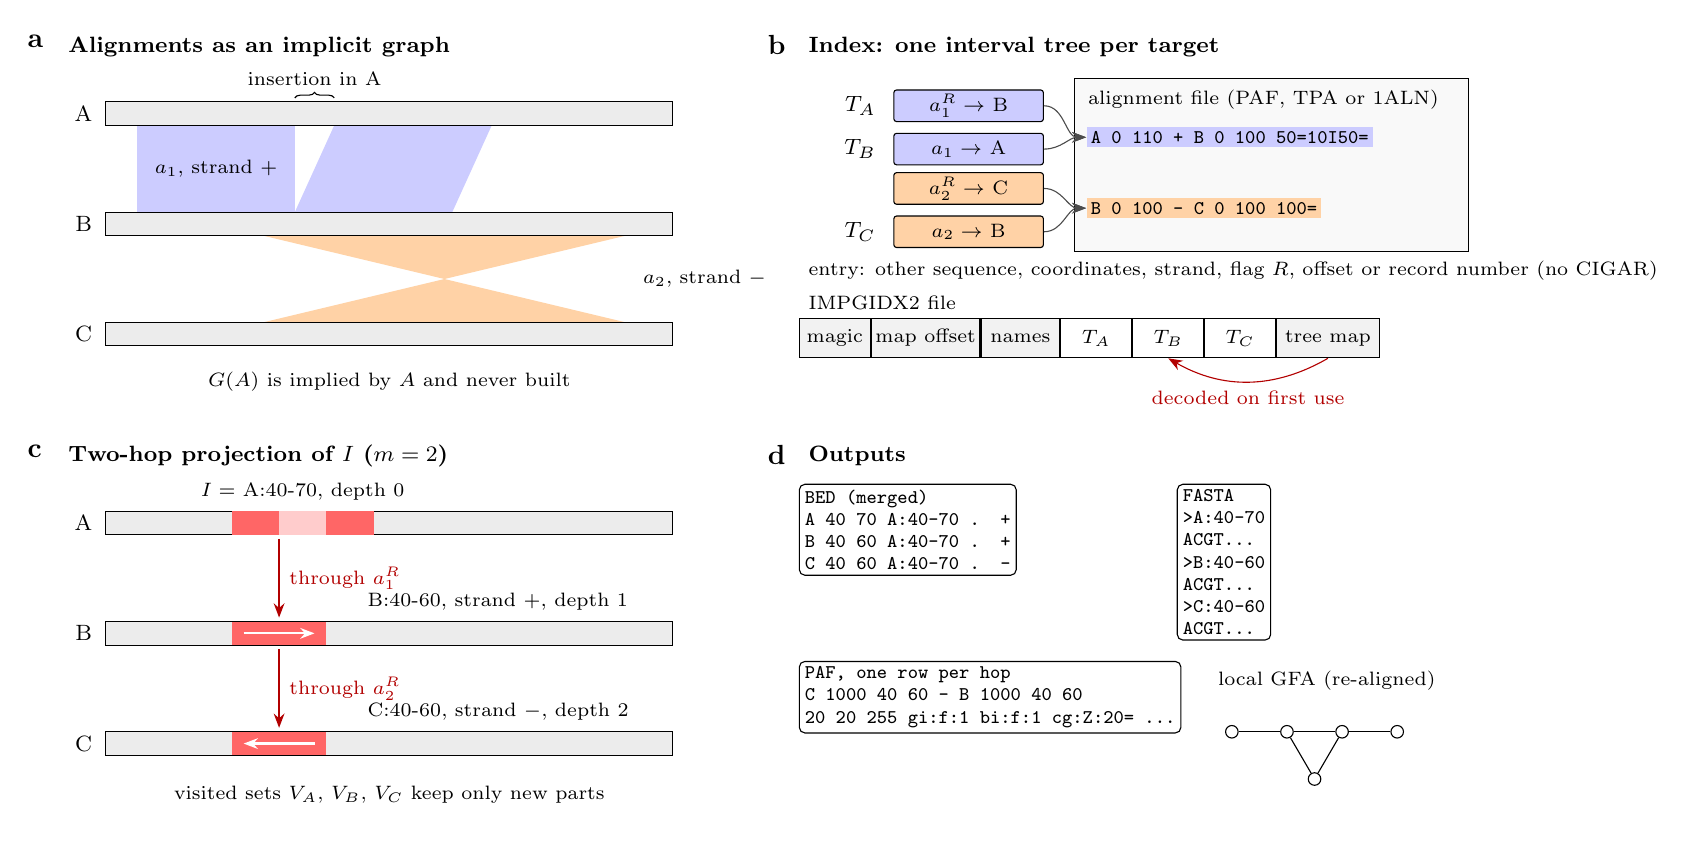
\begin{tikzpicture}[
  font=\footnotesize,
  >={Stealth[length=1.8mm]},
  bar/.style={draw, fill=gray!15},
  plab/.style={font=\bfseries\normalsize, anchor=north west, inner sep=0pt},
  ptitle/.style={font=\footnotesize\bfseries, anchor=west},
  entry/.style={draw, rounded corners=1pt, font=\scriptsize, minimum height=4mm, minimum width=19mm, inner sep=1.5pt, anchor=west},
  fline/.style={font=\ttfamily\scriptsize, anchor=west, inner sep=1.5pt},
  blk/.style={draw, fill=gray!10, minimum height=5mm, font=\scriptsize, inner sep=1.5pt},
  obox/.style={draw, rounded corners=2pt, fill=white, align=left, font=\ttfamily\scriptsize, inner sep=2pt, anchor=north west},
  hop/.style={->, thick, red!70!black},
]
%% panel a: sequences and alignments
\node[plab] at (0,9.95) {a};
\node[ptitle] at (0.4,9.8) {Alignments as an implicit graph};
\fill[blue!20] (1.4,8.8) -- (3.4,8.8) -- (3.4,7.7) -- (1.4,7.7) -- cycle;
\fill[blue!20] (3.9,8.8) -- (5.9,8.8) -- (5.4,7.7) -- (3.4,7.7) -- cycle;
\fill[orange!35] (3.0,7.4) -- (7.6,7.4) -- (3.0,6.3) -- (7.6,6.3) -- cycle;
\draw[bar] (1.0,8.8) rectangle (8.2,9.1);
\node[anchor=east] at (0.95,8.95) {A};
\draw[bar] (1.0,7.4) rectangle (8.2,7.7);
\node[anchor=east] at (0.95,7.55) {B};
\draw[bar] (1.0,6.0) rectangle (8.2,6.3);
\node[anchor=east] at (0.95,6.15) {C};
\draw[decorate, decoration={brace, amplitude=2pt}] (3.4,9.15) -- (3.9,9.15) node[midway, above=1pt, font=\scriptsize] {insertion in A};
\node[font=\scriptsize] at (2.4,8.25) {$a_1$, strand $+$};
\node[font=\scriptsize, anchor=west] at (7.7,6.85) {$a_2$, strand $-$};
\node[font=\scriptsize] at (4.6,5.55) {$G(A)$ is implied by $A$ and never built};
%% panel b: index
\node[plab] at (9.4,9.95) {b};
\node[ptitle] at (9.8,9.8) {Index: one interval tree per target};
\node[anchor=east] at (10.9,9.05) {$T_A$};
\node[entry, fill=blue!20] (eA) at (11.0,9.05) {$a_1^{R}\to$ B};
\node[anchor=east] at (10.9,8.5) {$T_B$};
\node[entry, fill=blue!20] (eB1) at (11.0,8.5) {$a_1\to$ A};
\node[entry, fill=orange!35] (eB2) at (11.0,8.0) {$a_2^{R}\to$ C};
\node[anchor=east] at (10.9,7.45) {$T_C$};
\node[entry, fill=orange!35] (eC) at (11.0,7.45) {$a_2\to$ B};
\draw[fill=gray!5] (13.3,7.2) rectangle (18.3,9.4);
\node[font=\scriptsize, anchor=north west] at (13.35,9.38) {alignment file (PAF, TPA or 1ALN)};
\node[fline, fill=blue!20] (r1) at (13.45,8.65) {A 0 110 + B 0 100 50=10I50=};
\node[fline, fill=orange!35] (r2) at (13.45,7.75) {B 0 100 - C 0 100 100=};
\draw[->, gray!60!black] (eA.east) to[out=0, in=180] (r1.west);
\draw[->, gray!60!black] (eB1.east) to[out=0, in=180] (r1.west);
\draw[->, gray!60!black] (eB2.east) to[out=0, in=180] (r2.west);
\draw[->, gray!60!black] (eC.east) to[out=0, in=180] (r2.west);
\node[font=\scriptsize, anchor=west] at (9.8,6.95) {entry: other sequence, coordinates, strand, flag $R$, offset or record number (no CIGAR)};
\node[font=\scriptsize, anchor=west] at (9.8,6.55) {IMPGIDX2 file};
\node[blk, minimum width=9mm, anchor=west] (m1) at (9.8,6.1) {magic};
\node[blk, minimum width=13mm, right=0pt of m1] (m2) {map offset};
\node[blk, minimum width=10mm, right=0pt of m2] (m3) {names};
\node[blk, minimum width=9mm, fill=white, right=0pt of m3] (m4) {$T_A$};
\node[blk, minimum width=9mm, fill=white, right=0pt of m4] (m5) {$T_B$};
\node[blk, minimum width=9mm, fill=white, right=0pt of m5] (m6) {$T_C$};
\node[blk, minimum width=13mm, right=0pt of m6] (m7) {tree map};
\draw[->, red!70!black] (m7.south) to[out=-150, in=-30] node[below, font=\scriptsize] {decoded on first use} (m5.south);
%% panel c: two-hop closure
\node[plab] at (0,4.75) {c};
\node[ptitle] at (0.4,4.6) {Two-hop projection of $I$ ($m=2$)};
\draw[bar] (1.0,3.6) rectangle (8.2,3.9);
\node[anchor=east] at (0.95,3.75) {A};
\draw[bar] (1.0,2.2) rectangle (8.2,2.5);
\node[anchor=east] at (0.95,2.35) {B};
\draw[bar] (1.0,0.8) rectangle (8.2,1.1);
\node[anchor=east] at (0.95,0.95) {C};
\fill[red!60] (2.6,3.6) rectangle (4.4,3.9);
\fill[red!20] (3.2,3.6) rectangle (3.8,3.9);
\node[font=\scriptsize, anchor=south] at (3.5,3.92) {$I=$ A:40-70, depth 0};
\fill[red!60] (2.6,2.2) rectangle (3.8,2.5);
\draw[->, white, thick] (2.75,2.35) -- (3.65,2.35);
\node[font=\scriptsize, anchor=south west] at (4.2,2.52) {B:40-60, strand $+$, depth 1};
\fill[red!60] (2.6,0.8) rectangle (3.8,1.1);
\draw[->, white, thick] (3.65,0.95) -- (2.75,0.95);
\node[font=\scriptsize, anchor=south west] at (4.2,1.12) {C:40-60, strand $-$, depth 2};
\draw[hop] (3.2,3.55) -- node[right, font=\scriptsize] {through $a_1^{R}$} (3.2,2.55);
\draw[hop] (3.2,2.15) -- node[right, font=\scriptsize] {through $a_2^{R}$} (3.2,1.15);
\node[font=\scriptsize] at (4.6,0.3) {visited sets $V_A$, $V_B$, $V_C$ keep only new parts};
%% panel d: outputs
\node[plab] at (9.4,4.75) {d};
\node[ptitle] at (9.8,4.6) {Outputs};
\node[obox] at (9.8,4.25) {BED (merged)\\A 40 70 A:40-70 . +\\B 40 60 A:40-70 . +\\C 40 60 A:40-70 . -};
\node[obox] at (14.6,4.25) {FASTA\\>A:40-70\\ACGT...\\>B:40-60\\ACGT...\\>C:40-60\\ACGT...};
\node[obox] at (9.8,2.0) {PAF, one row per hop\\C 1000 40 60 - B 1000 40 60\\20 20 255 gi:f:1 bi:f:1 cg:Z:20= ...};
\node[font=\scriptsize, anchor=west] at (15.0,1.75) {local GFA (re-aligned)};
\node[draw, circle, inner sep=1.6pt, fill=white] (g1) at (15.3,1.1) {};
\node[draw, circle, inner sep=1.6pt, fill=white] (g2) at (16.0,1.1) {};
\node[draw, circle, inner sep=1.6pt, fill=white] (g3) at (16.7,1.1) {};
\node[draw, circle, inner sep=1.6pt, fill=white] (g4) at (17.4,1.1) {};
\node[draw, circle, inner sep=1.6pt, fill=white] (g5) at (16.35,0.5) {};
\draw (g1) -- (g2) -- (g3) -- (g4);
\draw (g2) -- (g5) -- (g3);
\end{tikzpicture}%
}
\caption{The implicit pangenome graph in impg.
(a) Three sequences A, B and C, which stand for PanSN names such as \texttt{HG1\#1\#chr1}, and two pairwise alignments.
Alignment $a_1$ lies on the plus strand and has a 10 bp insertion in A, and $a_2$ lies on the minus strand (crossed band).
The alignments imply the variation graph $G(A)$ that seqwish would induce, and impg never builds it.
(b) The index keeps one interval tree per sequence.
Each alignment enters the tree of its target and, with the REVERSED flag $R$, the tree of its query.
An entry stores coordinates, strand, the flag and an offset or record number in the alignment file, and never a CIGAR.
The IMPGIDX2 file stores the names, one block per tree and a trailing tree map, and a query decodes only the trees it touches.
(c) A query at depth $m=2$.
The interval A:40-70 projects through $a_1$ to B:40-60, because the 10 inserted bases of A (light red) have no partner in B.
B:40-60 projects through $a_2$ to C:40-60 on the minus strand, and back to A:40-70, which is already visited.
White arrows show the strand.
(d) Outputs of \texttt{query} for this example.
BED rows are merged, and FASTA holds the input interval and the projected intervals.
PAF has one row per hop with its CIGAR slice, after touching or overlapping rows of one sequence pair merge.
The local GFA comes from aligning the intervals again.
File rows in b show query, start, end, strand, target, start, end and CIGAR.
Record $a_1$ is the fixture at tests/test\_transitive\_integrity.rs:462, and $a_2$ is not a fixture.
Coordinates in c and d follow the code with \texttt{-x -m 2 -d 0} and \texttt{-{}-min-transitive-len 0} (derived, not run).}
\label{fig:overview}
\end{figure*}
% src (legend): tests/test_transitive_integrity.rs:462 (a1 fixture); src/impg.rs:142-162 (inverted CIGAR), 164-211 (entry fields), 1686-1712 (two entries), 1758-1954 (IMPGIDX2 and lazy load), 2379-2628 (BFS), 2791-2929 (projection); src/paf.rs:171 (PAF CIGAR offset), src/tpa_parser.rs:116 (TPA record number), src/onealn.rs:697 (1ALN alignment index); src/main.rs:12055-12098 (BED), 12204 and 12648-12760 (PAF merge of contiguous or overlapping rows), 12236-12295 (PAF fields, gi:f and bi:f before cg:Z), 7629 and 7641-7643 (input interval removed for BEDPE and PAF only), 7749-7760 and 12487-12500 (FASTA keeps the input interval), 12324-12340 (GFA by re-alignment); impg query --help (-x, -d required, -m default 2); src/main.rs:4259; hop coordinates derived by hand from src/impg.rs:2791-2929

\textbf{Index.}
impg keeps one interval tree from the coitrees library \citep{Jones2024coitrees} per target sequence (Fig. \ref{fig:overview}b).
% src: src/impg.rs:226, 498-508, 1729-1737; Cargo.lock (coitrees 0.4.0)
An entry holds the other sequence, both coordinate pairs as 32-bit integers, a file number, a data length and one 64-bit word.
% src: src/impg.rs:164-174
Bit 63 of the word is the strand, bit 62 a REVERSED flag, and the rest the CIGAR byte offset or the tracepoint record number.
% src: src/impg.rs:178-207; src/alignment_record.rs:3-10
For bgzipped PAF the offset is a BGZF virtual offset.
% src: src/paf.rs:235-253, 286-298
The index stores no CIGAR and no sequence.
% src: src/impg.rs:164-174
A record with different query and target enters the tree of its target and, flagged REVERSED with swapped coordinates, the tree of its query.
% src: src/impg.rs:1686-1712
Self-alignments enter once, and \texttt{-{}-unidirectional} turns the second insertion off.
% src: src/impg.rs:1688; impg index --help (--unidirectional)
A query on any sequence therefore reaches every alignment that touches it.
% src: src/impg.rs:1686-1712; tests/test_transitive_integrity.rs:226-290
The index refers to alignment files by number, so a query must list them in the order used to build it.
% src: src/impg.rs:1657-1675 (file_index from enumerate); plan.md section 9 (code fix C4)
This paper uses one combined index (\texttt{-i}), not the per-file mode that 100 or more files select by default.
% src: src/main.rs:11277-11291; plan.md section 10

\textbf{On-disk format.}
An IMPGIDX2 file holds an 8-byte magic, the offset of a trailing tree map, the sequence names and lengths, and one block per tree.
% src: src/impg.rs:1758-1825
Loading reads the names and the tree map, and a query decodes a tree when it first touches its sequence.
% src: src/impg.rs:1827-1888, 1891-1954
Decoded trees stay in memory until the process ends, except in \texttt{stats}.
% src: src/impg.rs:1861-1865; eviction only at src/main.rs:13302, 13374

\textbf{Projection.}
For PAF input, impg reads the CIGAR at the stored offset and walks it once, up to the end of the requested range.
% src: src/impg.rs:599-656, 2829-2835
A REVERSED entry walks the inverted CIGAR, with \texttt{I} and \texttt{D} swapped and the order reversed on the minus strand.
% src: src/impg.rs:142-162, 651-654
TPA \citep{Guarracino2026tpa} and 1ALN \citep{Myers2025fastga,Durbin2024onecode} files store tracepoints \citep{Kaushan2026tracepoints}.
% src: citation-keys.md (Guarracino2026tpa, Myers2025fastga, Durbin2024onecode, Kaushan2026tracepoints); src/tpa_parser.rs; src/onealn.rs
For them impg finds the overlapping tracepoint segments, fetches their sequence from FASTA or AGC \citep{Deorowicz2023agc} and rebuilds their CIGAR with WFA2 \citep{MarcoSola2021wfa}.
% src: src/impg.rs:43-71 (thread-local WFA2), 750-927 (segment scan), 1031-1204 (subset rebuild), 1206-1362; src/sequence_index.rs:15-17, 78-90
A hit whose tracepoints cannot be fetched or projected is dropped with a debug message only.
% src: src/impg.rs:1230-1236, 1247-1254, 1330-1338
\pending{E1}{percentage of identical sorted rows between TPA exact and PAF projection of the same records at -m 0, 1 and 2, and the number of dropped tracepoint hits}
\texttt{-{}-approximate} interpolates the boundary inside the first and last overlapping segment, without sequences or WFA2, for BED and BEDPE output.
% src: src/impg.rs:1421-1637; src/main.rs:7393-7408; impg query --help (--approximate)
\pending{E1}{boundary difference in bp between approximate and exact mode, and the wall time of both}
Algorithm \ref{alg:bfs} projects each depth in parallel threads and applies the results one by one in frontier order.
% src: src/impg.rs:2452-2533 (rayon par_iter with ordered collect), 2539-2591 (sequential loop)
\pending{E2}{whether query output is identical at -t 1, 4, 16 and 48}

\textbf{Outputs.}
\texttt{query} writes BED, BEDPE, PAF, FASTA, GFA, VCF and MAF, and PAF rows keep the CIGAR slice of each hop (Fig. \ref{fig:overview}d).
% src: impg query --help (Output formats); src/main.rs:7614-7760, 12276-12295 (PAF fields cg:Z, gi:f, bi:f, an:Z)
Only BED output and one POA-engine GFA case have tests on the alignment backend.
% src: VERIFY_CORRECTIONS.md (core-index-projection, query output formats); tests/test_transitive_integrity.rs; tests/test_graph_output_crush.rs:37-124 (only alignment-backend GFA output test, POA engine); tests/test_aligner_validation.rs:3-31 (-o gfa only for option rejection)
With \texttt{-o gfa}, impg merges the projected intervals, drops their CIGARs and builds a graph of their sequences from scratch.
% src: src/main.rs:12324-12340; src/lib.rs:926-951
The default engine aligns the intervals with each other, induces a graph with an embedded seqwish \citep{Garrison2023seqwish}, smooths it \citep{Garrison2025smoothxg}, normalizes it with GFAffix \citep{Doerr2026gfaffix} and sorts it \citep{Garrison2026gfasort}.
% src: src/lib.rs:44-45, 1112-1131; src/smooth.rs:1-5 (smoothxg-style smoothing); impg query --help (--gfa-engine default pggb); citation-keys.md:17, 19
These graphs come from new alignments, so they need not match any part of $G(A)$.
% src: src/main.rs:12324-12340; plan.md section 11
The embedded seqwish also drops matches shorter than 23 bp by default, which violates the condition of Proposition \ref{prop:restrict}.
% src: impg query --help (--min-match-len default 23)
\authornote{Decision D4 (code fix C15): build -o gfa graphs from the projected PAF records, so that Proposition 2 can apply to them, or keep re-alignment and say so.}

\textbf{Partition and refine.}
\texttt{partition} picks unassigned bases, by default the longest unassigned region, and cuts them into windows of \texttt{-w} bp.
% src: src/commands/partition.rs:754-797 (longest mode), 948-972 (windows); impg partition --help (--selection-mode default longest)
A tail shorter than \texttt{-w} joins the previous window.
% src: src/commands/partition.rs:957-966
It computes the closure of each window with assigned bases masked.
% src: src/commands/partition.rs:369-397 (masked BFS)
Each closure is merged at \texttt{-d} and extended to sequence ends closer than 3,000 bp, and its unmasked part becomes one partition.
% src: src/commands/partition.rs:421-444 (merge_overlaps, extend_to_close_boundaries), 446-451 (mask), 1428-1466; impg partition --help (-d required, --min-boundary-distance default 3000)
By default, singleton partitions are then moved into a flanking partition.
% src: src/commands/partition.rs:31-46, 673-678; impg partition --help (--no-rehome-singletons)
The loop ends for any window of at least 1 bp (Supplementary Note S4).
% src: src/commands/partition.rs:1037-1380; Supplementary Note S4
\pending{E9}{partitions, uncovered bp and bp assigned to more than one partition on ScRAP 142}
\texttt{refine} widens a locus in steps of 1,000 bp, by default up to half its length per side.
% src: impg refine --help (--extension-step 1000, --max-extension 0.5)
It keeps the extension that maximizes the sequences, haplotypes or samples (\texttt{-{}-pansn-mode}) that span both ends by at least 1,000 bp.
% src: impg refine --help (--span-bp 1000, --pansn-mode); src/main.rs:7933-7935 (default Sequence); src/commands/refine.rs:188-273
\pending{E10}{haplotypes spanning both ends before and after refine at TERT and IGKV6-21, and the bp added per side}

\textbf{Memory.}
A build holds every alignment record (56 bytes of fields) and every tree entry (48 bytes) at once.
% src: src/alignment_record.rs:12-21 (2 x u32 + 6 x 8-byte fields = 56 bytes); src/impg.rs:164-174 (40 bytes) plus coitrees Interval first and last (8 bytes); src/impg.rs:1657-1737
For the 389,234,668 HPRC release 2 records, if none is a self-alignment, that is at least 59,163,669,536 bytes by field sizes, not by measurement.
% src: plan.md section 4 (records summed from the 466 TPA headers); 389,234,668 x 56 + 778,469,336 x 48 = 59,163,669,536, recomputed with python3 in this step
\pending{E2}{index build wall time, CPU time, peak RSS and index bytes for the 466 TPA files on the named node}
A code comment puts one AGC decompressor slot at 3.70 GB for the 3.30 GB HPRC archive, with up to 8 slots by default.
% src: src/agc_index.rs:58-83 (default 8, capped by the thread count), 87-100 (comment, 3.70 GB per slot)
Coordinates are 32-bit and operation lengths 29-bit, so impg does not support sequences above 2,147,483,647 bp or operations above 536,870,911 bp.
% src: src/impg.rs:81-109 (29-bit op length), 164-174 (i32); plan.md section 9 (code fix C13, no check today)

\section{The HPRC release 2 implicit pangenome}
\label{sec:release}

The Human Pangenome Reference Consortium release 2 (HPRC r2) also provides the alignments behind its PGGB graph through impg \citep{HPRC2026resources,Garrison2024pggb}.
% src: phase1/web/hpp_readme.md:151 (HPRC2026resources): "that same all-vs-all alignment is also provided through IMPG (implicit pangenome)"
The release README calls these alignments all-vs-all, although they do not cover every haplotype pair.
% src: phase1/web/hpp_readme.md:149, 151 ("all-vs-all alignment"); scripts/fig2_release.py stdout "ordered pairs 25221 of 216690 = 11.6392%", "unordered pairs 23738 of 108345 = 21.9096%"
\authornote{Disclose who produced the HPRC r2 IMPG files. The release README (lines 149 to 191) names no producer (plan.md question Q4).}
The release ships one tracepoint (TPA) file per target haplotype, 466 files in total \citep{Kaushan2026tracepoints,Guarracino2026tpa}.
% src: phase1/web/hpp_readme.md:183 "one file per haplotype, 466 total"; data/s3_tpas.xml KeyCount 466; per target: GRCh38 TPA and per-target PAF both hold 8,916,633 records (plan.md section 4, proposal-nm-brief.md section 2)
The 466 files hold 389,234,668 alignment records in 25,070,431,026 bytes (Table~\ref{tab:datasets}).
% src: scripts/fig2_release.py stdout "files 466 bytes 25070431026 records 389234668" (bytes from data/s3_tpas.xml, records from the TPA headers in data/strtab)
They comprise 460 HPRC r2 haplotype files from 230 samples, plus GRCh38 and CHM13.
% src: scripts/fig2_release.py stdout "composition {'reference': 2, 'hprc_r2': 460, 'genbank': 2, 'hg002': 2} hprc_r2 samples 230"; stems in data/partners.tsv column 1 (hprc_r2: 104 hap1, 104 hap2, 126 mat, 126 pat)
The other four files hold the maternal and paternal assemblies of HG06807 (v1.0, GenBank) and HG002 (v1.1).
% src: data/partners.tsv column 1 stems HG06807_mat_v1.0.genbank, HG06807_pat_v1.0.genbank, hg002v1.1.mat_MT.PanSN, hg002v1.1.pat.PanSN
All 466 headers declare Standard tracepoints and the edit-distance complexity metric with a maximum of 128.
% src: scripts/fig2_release.py stdout "encoding ... ('Standard', 'edit-distance', 128, ('gap-affine-2p', 5, 8, 2, 24, 1)): 466"; header layout ~/.cargo/git/checkouts/tpa-b0b145821a2566b9/f21b012/src/format.rs:869-947

We read the sequence names in each string table to list the haplotypes that each file aligns (Fig.~\ref{fig:release}).
% src: scripts/fig2_release.py parse_tpa_prefix (string table layout: tpa f21b012 src/format.rs:1244-1270)
The GRCh38 and CHM13 files each align all 465 other haplotypes.
% src: scripts/fig2_release.py stdout "reference GRCh38#0 ... partners 465", "reference CHM13#0 ... partners 465"; data/partner_summary.txt:1
Each assembly file aligns 35 to 74 other haplotypes, with a median of 52 (Fig.~\ref{fig:release}a).
% src: scripts/fig2_release.py stdout "assembly files 464 partners min 35 ... max 74 ... median 52.0"; data/partner_summary.txt:2
Together the files store 25,221 of the 216,690 ordered haplotype pairs (11.6392\%).
% src: scripts/fig2_release.py stdout "ordered pairs 25221 of 216690 = 11.6392%"; data/partner_summary.txt:3; data/pairs_out.txt:1
By default the index inserts each alignment in both directions, so a pair stored in either file is walked both ways.
% src: /home/guarracino/git/impg 0987752 src/impg.rs:1686-1709 (ENTRY 2 "if bidirectional && record.query_id != record.target_id", self-alignments skipped); src/main.rs:4085-4090 (--unidirectional turns it off, default bidirectional); src/main.rs:11277-11312 (same flag for per-file index, auto-selected at >= 100 files, and single index)
The index thus connects 23,738 of the 108,345 unordered pairs (21.9096\%).
% src: scripts/fig2_release.py stdout "unordered pairs 23738 of 108345 = 21.9096%"; data/pairs_out.txt:3
For 1,483 of these pairs, both files store alignments \pending{E1b}{index entries against twice the records for one such pair, count}.
% src: scripts/fig2_release.py stdout "ordered pairs present in both files 2966 unordered 1483"; data/pairs_out.txt:2
GRCh38 appears as a query in 45 of the 464 assembly files, and CHM13 in 51.
% src: scripts/fig2_release.py stdout "assembly files listing GRCh38#0 45 of 464", "listing CHM13#0 51 of 464"; data/pairs_out.txt:4
Without the two references, each assembly haplotype has 74 to 123 direct partners (median 98) and reaches all 463 others within 2 hops (Fig.~\ref{fig:release}c).
% src: scripts/fig2_release.py stdout "non-reference reach of 463: 1 hop min 74 ... max 123 ... median 98.0", "2 hops min 463 ... max 463"; data/pairs_out.txt:6-7
This reach counts haplotype pairs, not aligned bases \pending{E3}{bp reached per depth from non-reference regions with and without GRCh38 and CHM13 as bridges, percent of region bp}.
% src: plan.md section 5.4 (NOW for the pair graph, EXP for bases); E3
The release does not state how the aligned pairs were chosen \authornote{Ask the HPRC builders (plan.md question Q2). The wfmash:auto rule $10\ln(n)/n$ gives 13.1849\% at $n = 466$, against 11.2583\% observed for ordered pairs whose target is an assembly file (24,291 of 215,760).}.
% src: phase1/web/hpp_readme.md:149-191 (no pair rule stated); scripts/fig2_release.py stdout "nonref pairs 24291 of 215760 = 11.2583%" (fig2_release.py:207-209: all partners of the 464 assembly files over 464 x 465, references included as queries; without them 24195 of 214832 = 11.2623%, my arithmetic); judge-editor.md V8; sweepga 4713ce0 src/knn_graph.rs:202-215 (odgi-shredtools.md C item 8)

We make no storage claim.
% src: plan.md section 11
The TPA set is 3.918 times the size of the released GBZ v3 graph (25,070,431,026 vs 6,398,170,680 bytes).
% src: 25070431026 / 6398170680 = 3.918375 (my arithmetic); TPA bytes data/s3_tpas.xml; GBZ v3 bytes phase2/s3/pggb_wg.tsv (20250930_hprc25272.p98-k311.tmp.fix.v3.gbz)
TPA files plus the AGC sequence archive take 28,365,501,759 bytes before any impg index.
% src: 25070431026 + 3295070733 = 28365501759 (my arithmetic); AGC bytes `ls -la` /home/guarracino/git/impg/data/hprcv2/HPRC_r2_assemblies_0.6.1.agc
This is 4.433 times the GBZ v3 file and 0.840 times the GBZ v1 file (33,768,296,600 bytes).
% src: 28365501759 / 6398170680 = 4.433377, / 33768296600 = 0.840004 (my arithmetic); GBZ v3 and v1 bytes phase2/s3/pggb_wg.tsv
The Shredtools index hprcv2\_merged with its bumbl.bi file takes 27,478,774,573 bytes, and hprcv2\_enhanced\_merged takes 31,426,067,714 bytes.
% src: phase2/gi_all.xml (s3://genome-idx/mumemto/hprc/) hprcv2_merged.bumbl 27424443909 + .bumbl.bi 54330664 = 27478774573; hprcv2_enhanced_merged.bumbl 31371728522 + .bumbl.bi 54339192 = 31426067714 (my arithmetic); the bucket also holds hprcv2, hprcv2_filt and hprcv2_enhanced_filt
The Shredtools web client queries an enhanced HPRC r2 index remotely by HTTP Range requests, which impg does not support \citep{Shivakumar2026shredtools}.
% src: paper.txt:473-481 (HTTP Range), 497 (Fig. 5); odgi-shredtools.md B3 Fig. 5 "HPRCr2 (enhanced) index"; odgi-shredtools.md section C item 7 (no HTTP code in impg)
Table~\ref{tab:semantics} lists what each regional operation takes, returns and guarantees.

\begin{table*}[!t]
\caption{\label{tab:datasets}Datasets used in this paper.
Bytes are object sizes from anonymous S3 listings on 2026-11-08, or file sizes on disk for the AGC archive and the test fixture.
Records and partners come from the TPA headers and string tables (scripts/fig2\_release.py).
All 466 TPA headers also store the two-piece gap-affine penalties 5 (mismatch), 8 and 2 (first gap), and 24 and 1 (second gap).
R2 stands for s3://human-pangenomics/pangenomes/freeze/release2.}
% src: caption penalties from scripts/fig2_release.py stdout distance ('gap-affine-2p', 5, 8, 2, 24, 1); field order tpa f21b012 src/utils.rs:160-192
\centering
\footnotesize
% array package: loaded by bioinfo.cls:30
\setlength{\tabcolsep}{3pt}
\begin{tabular}{@{}>{\raggedright\arraybackslash}p{2.4cm}>{\raggedright\arraybackslash}p{3.0cm}>{\raggedright\arraybackslash}p{3.0cm}>{\raggedright\arraybackslash}p{4.6cm}>{\raggedright\arraybackslash}p{3.1cm}@{}}
\toprule
Name & Sequences or haplotypes & Bytes & Source & Use \\
\midrule
% src: data/s3_tpas.xml (466 keys, sum 25070431026); scripts/fig2_release.py stdout "records 389234668"; hpp_readme.md:191
HPRC r2 TPA set & 466 haplotypes, 389,234,668 records & 25,070,431,026 & \url{R2/impg/tpas/} \citep{HPRC2026resources} & Fig.~\ref{fig:release}, index and queries (E2, E3b, E8, E10) \\
% src: data/s3_tpas.xml GCA_000001405.15...tpa 560062985; phase2/s3_all-vs-1.xml GCA_...merged.paf.gz 6532446867; fig2_release.py stdout "reference GRCh38#0: bytes 560062985 records 8916633 partners 465"
GRCh38 star & 465 query haplotypes, 8,916,633 records & 560,062,985 (TPA), 6,532,446,867 (PAF.gz) & \url{R2/impg/tpas/} and \url{R2/impg/pafs/all-vs-1/} & TPA against PAF (E1), copies (E7), E3a \\
% src: data/s3_tpas.xml chm13v2.0...tpa 455391474; phase2/s3_all-vs-1.xml chm13...merged.paf.gz 5590178237; fig2_release.py stdout "reference CHM13#0: bytes 455391474 records 7149766 partners 465"
CHM13 star & 465 query haplotypes, 7,149,766 records & 455,391,474 (TPA), 5,590,178,237 (PAF.gz) & \url{R2/impg/tpas/} and \url{R2/impg/pafs/all-vs-1/} & GRCh38 to CHM13 projection (E3a) \\
% src: ls -la /home/guarracino/git/impg/data/hprcv2/HPRC_r2_assemblies_0.6.1.agc 3295070733; judge-feasibility.md section 1 (agc listset, 466 names equal the TPA stems)
HPRC r2 AGC archive & 466 AGC samples, one per TPA stem and named alike & 3,295,070,733 & \url{HPRC_r2_assemblies_0.6.1.agc} \citep{Deorowicz2023agc} \authornote{public URL} & Sequences for exact TPA projection and FASTA or GFA output \\
% src: phase2/s3/pggb_wg.tsv v3.gbz 6398170680, v1.gbz 33768296600; hpp_readme.md:151, 155 (same all-vs-all alignment, pggb -p 98 -k 311)
PGGB graph, GBZ v3 and v1 \citep{Siren2022gbz} & Built from the same alignment with pggb -p 98 -k 311 \authornote{haplotype count not checked} & 6,398,170,680 (v3), 33,768,296,600 (v1) & \url{R2/pggb/gfas/whole-genome/20250930_hprc25272.p98-k311.tmp.fix.v3.gbz} & vg chunk comparator (E2), consistency (E8) \\
% src: phase2/gi_all.xml (bucket genome-idx) hprcv2_merged.bumbl 27424443909, .bumbl.bi 54330664; paper.txt:101-102 (r2, N=476)
Shredtools HPRC r2 index & 476 genomes, as its authors count them & 27,478,774,573 (bumbl and bumbl.bi) & \url{s3://genome-idx/mumemto/hprc/hprcv2_merged.bumbl} \citep{Shivakumar2026shredtools} & Shredtools comparator (E2, E10) \\
% src: phase2/r1.xml chr19.hprc-v1.0-pggb.gfa.gz 345202999; judge-feasibility.md:37-38 (freeze1 README, pggb -n 90; 92-haplotype set cannot be rebuilt); paper.txt:285 (92 chr19 assemblies); plan.md E5 dataset line
HPRC year-1 chr19 PGGB graph & 90 haplotypes (pggb -n 90) & 345,202,999 (GFA.gz) & \url{s3://human-pangenomics/pangenomes/freeze/freeze1/pggb/chroms/chr19.hprc-v1.0-pggb.gfa.gz} \citep{Liao2023hprc} & Same 90-haplotype input for impg and Shredtools in E5, not the 92 haplotypes of \citet{Shivakumar2026shredtools} \\
% src: plan.md section 7 E4 (accessions and download path not checked); ODonnell2023scrap
ScRAP \textit{S. cerevisiae} & 142 strains \authornote{haplotype count not checked} & \authornote{not checked} & \citet{ODonnell2023scrap} \authornote{accessions} & Holdout never used for tuning (E4, E9) \\
% src: zcat /home/guarracino/git/impg/tests/test_data/yeast.chrV.fa.gz: 7 headers, 4029392 bp; ls -la 1254257 bytes; git ls-files (tracked, added in 46a0249)
Yeast chrV fixture & 7 sequences, 4,029,392 bp & 1,254,257 & \url{tests/test_data/yeast.chrV.fa.gz} in impg \citep{Guarracino2026impg} & Tests, local graph tuning (E6) \\
\bottomrule
\end{tabular}
\end{table*}

\begin{table*}[!t]
\caption{\label{tab:semantics}What each regional operation takes, returns and guarantees.
impg facts come from impg 0.5.0 help text and source at commit 0987752.
Shredtools facts come from its preprint \citep{Shivakumar2026shredtools}, and other tools from their help, usage text or README \citep{Guarracino2022odgi,Garrison2018vg,Kent2003chain,Kuhn2013ucsc,Hickey2013hal,Chin2023pgrtk}.
``Not stated'' means that we found no statement in those sources.}
\centering
\scriptsize
\setlength{\tabcolsep}{3pt}
\begin{tabular}{@{}>{\raggedright\arraybackslash}p{1.5cm}>{\raggedright\arraybackslash}p{2.5cm}>{\raggedright\arraybackslash}p{2.3cm}>{\raggedright\arraybackslash}p{3.5cm}>{\raggedright\arraybackslash}p{3.1cm}>{\raggedright\arraybackslash}p{1.3cm}>{\raggedright\arraybackslash}p{1.6cm}@{}}
\toprule
Operation & Input & Output & Boundary semantics & Multiple copies & Needs a graph & Remote access \\
\midrule
% src: phase2/plan_help_query.txt:169-174 (-d required), 191-192 (-x enables transitive queries), 187-203 (-m default 2, under transitive query options), 222-224 (--approximate bed/bedpe), 449-460 (formats); src/main.rs:12324-12340 (gfa re-aligns merged intervals); src/impg.rs:2574-2589 (self-hits not expanded); odgi-shredtools.md section C item 7 (no HTTP)
impg query & Indexed PAF, 1ALN or TPA alignments, an interval on any indexed sequence & BED, BEDPE, PAF, FASTA, MAF, and GFA or VCF from re-aligned intervals & Base-level projection of the query ends through each CIGAR. One hop by default, at most \texttt{-m} hops (default 2) with \texttt{-x}. \texttt{-{}-approximate} interpolates tracepoints for BED and BEDPE & One row per aligned interval. Rows within \texttt{-d} bp merge. Self-hits are not expanded & No & No \\
% src: phase2/plan_help_refine.txt:46 (-r), 49 (-b), 1 ("maximize the number of samples that span both ends"), 119-150 (--span-bp 1000, --max-extension 0.5, --extension-step 1000, --pansn-mode, --support-output); VERIFY_CORRECTIONS.md:64 (default sequence mode), :80 (8-column table)
impg refine & A locus (\texttt{-r} or BED) and the same index & 8-column table of refined loci, optional support BED & Extends each side in 1,000 bp steps, up to 0.5 of the locus, to maximize entities that span both ends by 1,000 bp & Counts sequences (default), samples or haplotypes, not copies & No & No \\
% src: phase2/plan_help_partition.txt:113-140 (-w, selection modes, --min-missing-size 3000), 183-186 (formats); phase1/partition-regional.md:11, 58, 86 (greedy windows, transitive queries, masking, first partition owns a base)
impg partition & The same index and a window size \texttt{-w} & Per-partition BED, GFA, VCF, MAF or FASTA & A window and its transitive homologs. Unassigned fragments under 3,000 bp join a neighbouring interval & The first partition that reaches a base owns it \pending{E9}{bp uncovered and bp owned twice on ScRAP 142} & No & No \\
% src: paper.txt:278-283, 602-608 (nearest flanking collinear multi-MUMs, bounds reported); odgi-shredtools.md B6 (0 to 328,599 bp in examples), B8 item 3 (466 of 476 in Fig. 5); paper.txt:473-481 (HTTP Range)
Shredtools extract & Multi-MUM index (bumbl, bumbl.bi), an interval on any genome (multi index) & Syntenic window per genome with bound distances, FASTA in the web tool & Window ends at the nearest flanking collinear multi-MUMs. The distance to each flank is reported as a bound & One window per genome. Its Fig. 5 shows 466 of 476 sequences for BRCA1 & No & Yes, HTTP Range requests \\
% src: paper.txt:437-444 (zoom flags outlier genomes), 461-463 (single copy per genome after enhance), 629-635 (enhance gaps, median - 5 x MAD exclusion); odgi-shredtools.md B3 Fig. 5 (enhanced index in the web tool)
Shredtools enhance, zoom & The index and the gap sequences between multi-MUMs & Local multi-MUMs merged into the index, and flagged outlier genomes & Local multi-MUMs shrink bounds. Zoom lets the user drop outlier genomes & Extracted regions tend to hold a single copy per genome & No & Enhanced index queried by HTTP \\
% src: paper.txt:108-111 (shred, unsplittable stretches); odgi-shredtools.md B4 (no graph built from shreds in the paper)
Shredtools shred & The multi-MUM index & Collinear homologous regions & Bounded by multi-MUMs. Marker coverage sets the size & Stretches without markers form one unsplittable region & No & Not stated \\
% src: odgi extract --help (odgi v0.9.4-82-g34c461ff): -r/-b path ranges find nodes, -c and -L default 0, -d default 300000, -p keeps a subset of paths; Guarracino2022odgi
odgi extract & ODGI or GFA graph, path range or BED & Subgraph (ODGI) & Nodes that the path range touches. Context steps and bases default to 0 & Paths through the extracted nodes are kept as subpaths. Subpaths within 300,000 bp merge & Yes & Not in help \\
% src: vg chunk --help (vg v1.76.1): -x graph or XG index, -p path range, -c context steps default 1, -O vg/pg/hg/gfa, -T with -G GBWT; Garrison2018vg
vg chunk & Graph or XG index, path range & Subgraph (vg, pg, hg, GFA) & Nodes in the path range plus 1 node step of context by default & Haplotype threads with \texttt{-T} and a GBWT & Yes & Not in help \\
% src: kent master 7fc350a src/hg/liftOver/liftOver.c:53-100 (usage: map.chain old genome target, new genome query; -minMatch; -multiple); src/hg/inc/liftOver.h:12 (LIFTOVER_MINMATCH 0.95); Kent2003chain, Kuhn2013ucsc
liftOver & BED (or GFF, genePred, PSL) and one chain file per ordered assembly pair & Lifted file and unmapped records & Bases mapped through chain blocks. By default a record fails if less than 0.95 of its bases remap & One output region. \texttt{-multiple} allows several & No & Not in usage \\
% src: hal master 227ff07 liftover/impl/halLiftoverMain.cpp:18-43 (noDupes, BED or PSL); hal README.md:140-147 (UDC), 337-341 ("base-by-base mapping ... following paralogy relations"); Hickey2013hal
halLiftover & HAL multiple alignment from Cactus, BED or PSL on one genome & BED or PSL on a target genome & Base-by-base mapping through alignment columns & Follows paralogy by default. \texttt{-{}-noDupes} turns it off & A HAL alignment & HTTP if built with UDC \\
% src: GeneDx/pgr-tk 5835435 pgr-bin/src/bin/pgr-query.rs:10-80 (AGC backend, k 56, w 80, r 4, merge_range_tol 100000), 205-280 (per sequence and strand hit merging); README.md:29-36; Chin2023pgrtk
PGR-TK pgr-query & Query sequence (FASTA), AGC-backed minimizer database & Hit summary (BED optional) and FASTA of hit regions & Ends of sparse minimizer alignments (k 56, w 80, r 4). Hits within 100,000 bp merge & Each hit region per sequence and strand is reported & No (MAP graph built later) & Not stated \\
\bottomrule
\end{tabular}
\end{table*}

\begin{figure*}[!t]
\centering
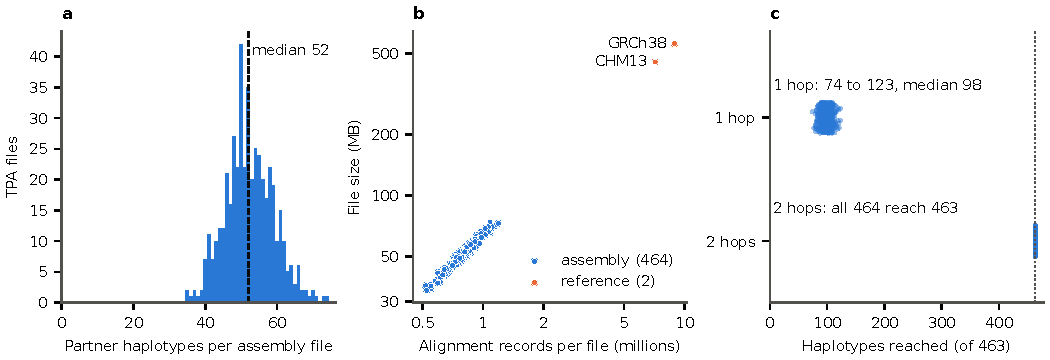
\includegraphics[width=\textwidth]{fig/fig2_release.pdf}
\caption{\label{fig:release}The HPRC r2 TPA files as an alignment network.
Each TPA file holds the alignments that target one haplotype, and its string table names every haplotype that the file aligns.
(\textbf{a}) Partner haplotypes per assembly file for the 464 assembly files.
Counts include GRCh38 and CHM13 where a file lists them (45 and 51 files).
The dashed line marks the median, 52.
The GRCh38 and CHM13 files list 465 partners each and are not shown.
(\textbf{b}) File size in the S3 listing against alignment records in the header, for all 466 files, on log axes.
The two reference files are labelled.
(\textbf{c}) Non-reference haplotypes reached from each of the 464 assembly haplotypes in the undirected pair graph without GRCh38 and CHM13.
One hop counts direct partners stored in either file, and two hops add their partners.
The dotted line marks all 463 others, and points are spread vertically for visibility.
Pairs come from sequence names, not from aligned bases, and E3 measures reach in bases.
Data are the 466 string tables and the S3 listing in data/, and the script is scripts/fig2\_release.py.}
% src: scripts/fig2_release.py stdout (panel a histogram, panel b ranges, panel c histograms); data/pairs_out.txt; data/partner_summary.txt
\end{figure*}

\section{Results}
\label{sec:results}

Each subsection states a question, its design and slots for its results.
All runs use one tagged impg build, and we store its sha256 digest, version and commit next to each result \authornote{tag name, Zenodo version DOI and owner of the frozen build, decision D6 and code fix C1}.
% src: supporting/plan.md section 7 (rules for every run) and section 9 C1
Every benchmark names its index with \texttt{-i}, which forces a single index.
% src: impg src/main.rs:11277-11291 (IndexMode::Auto returns single when an index path is given)
Without \texttt{-i}, impg switches to one index per file at 100 or more files, and no test covers that mode.
% src: impg src/main.rs:11281-11287; supporting/plan.md section 9 C6 (src/multi_impg.rs:757-952, 0 tests)
A fixed-seed sampler draws every region set, and held-out sets never choose parameters (Supplementary Note S5 and Table~\ref{tab:commands}).
% src: supporting/plan.md section 7 (rules for every run)

\subsection{Tracepoint projection and CIGAR projection}
\label{sec:res-tpa}

HPRC release 2 distributes the PGGB alignments as 466 TPA files, one per haplotype \citep{HPRC2026resources,Guarracino2026tpa}.
% src: HPRC2026resources, README lines 151 and 183 (phase1/web/hpp_readme.md:151, 183)
For tracepoint input, impg rebuilds the CIGAR of the segments that overlap a query from the sequences with WFA2 \citep{Kaushan2026tracepoints,MarcoSola2021wfa}.
% src: impg src/impg.rs:1206-1362
No test compares this path with PAF input, and impg drops a hit it cannot rebuild with only a debug message.
% src: supporting/plan.md section 9 C2; impg src/impg.rs:1230-1236, 1247-1254, 1330-1338, 1436-1442, 1453-1460
We ask whether exact tracepoint projection returns the same rows as CIGAR projection of the same alignments.
We use the GRCh38 target file, 8,916,633 records, as TPA (560,062,985 bytes) and as gzipped PAF (6,532,446,867 bytes).
% src: S3 listings of release2/impg/tpas and release2/impg/pafs/all-vs-1 (phase2/s3/tpas.tsv, phase2/s3/pafs.tsv); supporting/plan.md sections 4 and 5.4 (record counts equal); data/partners.tsv line 1
We project 1,000 random 10 kb GRCh38 regions, plus 200 held out, at depth 1, 2 and unbounded, without merging.
% src: supporting/plan.md section 7 E1
We count identical sorted BEDPE rows, rows found in one output only, the largest boundary shift and dropped tracepoint hits.
% src: supporting/plan.md section 7 E1
We also run \texttt{-{}-approximate}, which serves only BED and BEDPE output, without tuning it.
% src: impg query --help (--approximate)
A second test indexes two assembly files that list each other, with and without \texttt{-{}-unidirectional}, because both files store their alignments.
% src: data/pairs_out.txt (2,966 ordered pairs stored in both files); impg src/impg.rs:1686-1712 (each non-self record is also inserted reversed); supporting/plan.md section 7 E1b
Exact tracepoint and PAF projection gave \pending{E1}{identical sorted rows, \%, per depth and set}.
The tracepoint path dropped \pending{E1}{tracepoint hits, count}.
Approximate mode shifted boundaries by \pending{E1}{median and maximum shift, bp} at \pending{E1}{median s per query, both modes}.
The reciprocal pair gave \pending{E1}{index entries per record, merged BED identity}.
Every tracepoint result below depends on this test (Supplementary Fig.~S2).

\subsection{Indexing and querying the whole release}
\label{sec:res-release}

The Shredtools authors wrote that they could not compute a comparable impg index over whole HPRCr1 assemblies or the HPRCr2 collection of N = 476 \citep{Shivakumar2026shredtools}.
% src: Shivakumar2026shredtools, references/biorxiv-2026-07-03-736354/paper.txt:285-287
The same preprint states that impg in practice runs on a sparse sample of pairs, and it benchmarked 6\% and 17\% pair sets.
% src: Shivakumar2026shredtools, paper.txt:301-312
We ask whether the 389,234,668 released alignments index on one node, and what a regional query then costs.
% src: data/partners.tsv column 2 summed over 466 files
The 466 TPA files take 25,070,431,026 bytes, and the AGC sequence archive takes 3,295,070,733 bytes \citep{Deorowicz2023agc}.
% src: phase2/s3/tpas.tsv (sum); supporting/plan.md section 4 (local ls of HPRC_r2_assemblies_0.6.1.agc)
By the field sizes in the code, a single-index build holds at least 59,163,669,536 bytes in memory at once.
% src: impg src/main.rs:11621-11760 and src/impg.rs:1657-1735; supporting/plan.md section 4 (389,234,668 x 56 + 778,469,336 x 48)
We therefore build on one cluster node \authornote{node name, CPU model, RAM and scratch bytes, decision D5}.
We sample 1,000 regions each of 1 kb, 10 kb, 100 kb and 1 Mb on non-reference haplotypes, plus 200 held out per size.
% src: supporting/plan.md section 7 E2 (seed 2)
Each region runs as its own impg process on one thread, five times with a warm page cache, at depth 1 and 2.
% src: supporting/plan.md section 7 E2
Each run uses exact and approximate mode under \texttt{/usr/bin/time -v}.
A batch run of the 10 kb set at 1, 4, 16 and 48 threads measures throughput and output identity.
One query covers all of CHM13 chromosome 1.
vg chunk from vg v1.76.1 extracts each region from the GBZ version 3 file of the PGGB graph built from the same alignments \citep{Garrison2018vg,Siren2022gbz,Garrison2024pggb} \authornote{check that vg v1.76.1 reads GBZ version 3, which the release README says needs ``a recent release of vg'' without naming a version}.
% src: HPRC2026resources README line 151 (same all-vs-all alignment), line 159 (v3.gbz requires a recent release of vg); phase2/s3/pggb_wg.tsv (v3.gbz 6,398,170,680 bytes); vg version on the workstation; supporting/plan.md section 14 (v3 GBZ read by vg v1.76.1 not run)
Shredtools extract reads its public HPRC release 2 index, hprcv2\_merged.bumbl, which takes 27,478,774,573 bytes with its \texttt{.bi} file \citep{Shivakumar2026shredtools,Shivakumar2025mumemto}.
% src: phase2/judge-feasibility.md section 1 (aws s3 ls s3://genome-idx/mumemto/hprc/: hprcv2_merged.bumbl 27,424,443,909 + .bumbl.bi 54,330,664 bytes)
All three tools query the same 1,000 GRCh38 regions of 10 kb.
% src: supporting/plan.md section 7 E2
impg and Shredtools return intervals, and vg chunk returns a subgraph, so this comparison measures cost, not output.
Shredtools also answers queries from a web browser through HTTP Range requests on its cloud-hosted index, and impg has no remote access.
% src: paper.txt:25-26, 476, 501, 572 (HTTP Range requests), 640-641 (browser tool); supporting/plan.md section 10 (remote HTTP access not implemented)
impg pays no alignment cost here, because the PGGB build produced the alignments, and the release does not state that cost.
% src: HPRC2026resources README line 151; supporting/plan.md section 12 Q3
The build gave \pending{E2}{outcome, wall and CPU h, peak RSS GB, index bytes} (Fig.~\ref{fig:cost}a).
Per-query cost was \pending{E2}{median and p95 s, peak RSS GB, per size, depth and mode} (Fig.~\ref{fig:cost}b).
On the shared GRCh38 regions, vg chunk took \pending{E2}{median and p95 s, peak RSS GB}.
Shredtools took \pending{E2}{median and p95 s, peak RSS GB} on the same regions.
The whole-chromosome query took \pending{E2}{s and peak RSS GB, or the limit reached}.
Batch output across thread counts was \pending{E2}{identical or not, differing rows} (Fig.~\ref{fig:cost}d).
We make no storage claim.
Exact tracepoint queries need the AGC archive, and GBZ stores the sequences itself.
% src: impg 0987752 src/main.rs:4186-4215 (tracepoint files need --sequence-files unless --approximate with bed or bedpe)
The TPA set and the AGC archive take 28,365,501,759 bytes, 4.433 times the 6,398,170,680 bytes of GBZ version 3, before any impg index (Fig.~\ref{fig:cost}c).
% src: 25,070,431,026 + 3,295,070,733 = 28,365,501,759; 28,365,501,759 / 6,398,170,680 = 4.433 (phase2/s3/tpas.tsv, phase2/s3/pggb_wg.tsv, supporting/plan.md section 4)
As a consistency check, we compare impg intervals at depth 2 with vg chunk path intervals on 1,000 GRCh38 and 1,000 non-reference regions.
% src: supporting/plan.md section 7 E8 (seed 10)
The PGGB graph drops exact matches shorter than 311 bp, so this check measures consistency, not truth \citep{Garrison2023seqwish,Garrison2024pggb}.
% src: HPRC2026resources README line 155 (pggb -p 98 -k 311)
Per-region base-pair Jaccard was \pending{E8}{median and IQR, segmental duplication, satellite and other strata} (Supplementary Fig.~S3).

\begin{figure}[!tpb]
\centering
\fbox{\parbox{0.95\linewidth}{\small Planned panels.
(a) Index build cost of the 466 TPA files.
(b) Per-query wall time and peak memory by region size for impg, vg chunk and Shredtools.
(c) Bytes on disk of released and derived files.
(d) Batch wall time and output identity by thread count.}}
\caption[Cost on the whole release]{\textbf{Cost on the whole release.}
(a) Index build of the 466 HPRC release 2 TPA files in single-index mode.
Bars give wall time (h), CPU time (h), peak resident memory (GB) and index size (bytes), each axis from 0.
Data from E2, \texttt{/usr/bin/time -v} on the node of Supplementary Note S5.
(b) Per-query wall time (s, y axis from 0) against region size (x axis, 1 kb, 10 kb, 100 kb and 1 Mb).
Points are medians and bars are 95th percentiles of 1,000 regions times 5 replicates.
Series are impg exact and approximate at depth 1 and 2, vg chunk on GBZ version 3, and Shredtools extract on hprcv2\_merged.bumbl.
The vg and Shredtools series use the 1,000 GRCh38 regions of 10 kb.
A second row gives peak resident memory (GB, y axis from 0).
Data from E2.
(c) Bytes on disk (y axis from 0) of eight files or sets.
These are the per-target PAF.gz set, the TPA set, the AGC archive (3,295,070,733 bytes), the impg index, GBZ versions 1 and 3, the gbz-base database and the Shredtools index.
Data from the S3 listings of 2026-11-08 and, for the impg index, from E2.
(d) Batch wall time (s, y axis from 0) against threads (x axis, 1, 4, 16 and 48) for 1,000 non-reference 10 kb regions.
Marks flag thread counts whose output differs from the 1-thread output.
Data from E2.}
\label{fig:cost}
\end{figure}

\subsection{Reach and reference dependence}
\label{sec:res-reach}

Every assembly in the release aligns to GRCh38 and CHM13, whose two files list all 465 other haplotypes \citep{Schneider2017grch38,Nurk2022chm13}.
% src: data/partner_summary.txt (refs 465 each); data/pairs_out.txt
Between non-reference haplotypes, the index walks 22,809 of 107,416 unordered pairs (21.2343\%).
% src: data/pairs_out.txt
At the level of pairs, every non-reference haplotype reaches all 463 others within two hops without either reference (Fig.~\ref{fig:release}c).
% src: data/pairs_out.txt (2 hops min 463 median 463); sections/04.release.tex fig:release panel c
Pair-level reach does not measure bases, so we ask how many bases a query reaches without the two references.
We also ask how well transitive projection recovers a held-out direct alignment.
In the first test we project 1,000 random 1 kb GRCh38 regions to CHM13, plus 200 held out.
% src: supporting/plan.md section 7 E3a (seed 3)
One index holds the GRCh38 and CHM13 target files, and a second index holds them without the direct GRCh38 and CHM13 records.
% src: supporting/plan.md section 7 E3a
The second index reaches CHM13 only through other haplotypes, at depth 2 and 3.
We score it against the direct projection and against a public GRCh38-to-CHM13 chain file \citep{Kent2003chain} \authornote{choose the chain file and record its provenance}.
In the second test we choose 10 non-reference haplotypes, each with one partner whose alignments only the haplotype's own file stores.
% src: supporting/plan.md section 7 E3b (seed 4); data/pairs_out.txt (2,966 of 25,221 ordered pairs are stored in both files)
We replace each such file by its per-target PAF without the partner's records, so no direct alignment links the two.
% src: supporting/plan.md section 7 E3b
We query 100 random 10 kb regions per haplotype, 20 of them held out, at depth 1, 2, 3, 4 and unbounded.
% src: supporting/plan.md section 7 E3b
Each depth runs with the references and without them, through a subset list that removes GRCh38 and CHM13 as outputs and as bridges.
% src: impg src/impg.rs:2496-2505 (subset filter applied before a projection joins the next frontier); VERIFY_CORRECTIONS.md:18
The truth is the direct projection of the same regions on the full index.
At depth 1 no direct alignment remains, so this depth serves as a control.
Metrics are bp recall, bp precision, the exact-boundary rate at 0, 1, 10 and 100 bp, and bases reached per depth.
% src: supporting/plan.md section 7 E3
Strand agreement waits for the strand decision, because impg sets BED strand per hop and does not compose it back to the query.
% src: impg src/impg.rs:282-286 and src/main.rs:12072-12079; supporting/plan.md sections 9 C7 and 13 D3
GRCh38 to CHM13 projection through haplotypes gave \pending{E3}{bp recall and precision against direct projection and against the chain, depth 2 and 3}.
Held-out partner recall was \pending{E3}{median per-region bp recall with and without references, per depth} (Fig.~\ref{fig:recall}c).
Bases reached were \pending{E3}{bp per depth, with and without references} \authornote{Fig.~\ref{fig:release} has panels a to c only. Choose the panel that shows bases reached per depth}.
We report unbounded runs that do not finish with their limit.

\subsection{Sparse alignment sets and transitive error}
\label{sec:res-sparse}

The number of genome pairs grows as $n(n-1)/2$, so 90 haplotypes give 4,005 pairs and 142 strains give 10,011.
We ask how much homology transitive projection recovers, by depth, as the fraction of aligned pairs falls.
The tuning set is the all-pairs chr19 alignment of 90 HPRC year-1 haplotypes from Section~\ref{sec:res-genes} \citep{Liao2023hprc}.
% src: supporting/plan.md section 7 E4 and E5
The holdout is the ScRAP set of 142 \textit{Saccharomyces cerevisiae} assemblies, which never sets a parameter \citep{ODonnell2023scrap}.
% src: supporting/plan.md section 7 E4; ODonnell2023scrap
We align all pairs with wfmash through \texttt{impg align} and keep its default filters \citep{Guarracino2024wfmash,Garrison2026sweepga}.
% src: impg align --help (--sparsify none default, plane-sweep and scaffold filters on by default)
From each all-pairs set we draw four subsets of pairs.
Two are random 6\% and 17\% subsets, the two pair fractions of the Shredtools benchmark \citep{Shivakumar2026shredtools}.
% src: paper.txt:301-303 (6% of pairwise alignments), 310-311 (17%, the default auto setting); the preprint gives no selection rule for either set
The third holds the pairs that \texttt{-{}-sparsify auto} selects, and the fourth is a star to one genome fixed in advance.
% src: supporting/plan.md section 7 E4; section 13 D8 (hub strain)
Above 50 haplotypes, \texttt{auto} keeps the 5 nearest and 2 farthest Mash neighbours of each haplotype plus a 0.05 random fraction of pairs \citep{Ondov2016mash}.
% src: sweepga 4713ce0 src/knn_graph.rs:514-532 (auto rule) and 243-280 (tree pairs)
impg groups FASTA records by PanSN haplotype before this step, and it always aligns contigs within one haplotype.
% src: impg src/commands/align.rs:147-179; sweepga 4713ce0 src/knn_graph.rs:589-618 (within-haplotype pairs always added), 636-677 (haplotype-level selection)
We draw the random subsets in the harness with a fixed seed, because \texttt{random:<f>} keeps each pair by a hash threshold.
% src: sweepga 4713ce0 src/knn_graph.rs:371-392
We record whether the \texttt{auto} pair count at commit 0987752 matches the 17\% that Shredtools called the default auto setting of impg v0.4.0.
% src: paper.txt:310-311 (default auto setting), 838-839 (impg v0.4.0); sweepga 4713ce0 src/knn_graph.rs:514-532, pinned in Cargo.lock at 0987752
The truth is direct projection on the all-pairs index.
We project 1,000 random 10 kb regions per set at depth 1, 2, 3, 4 and unbounded on each subset index.
% src: supporting/plan.md section 7 E4 (seed 5)
Metrics are bp recall, bp precision, the exact-boundary rate at 0, 10 and 100 bp, and haplotypes reached.
We also report pairs aligned and alignment CPU time per subset.
On chr19, recall at depth 2 was \pending{E4}{median per-region bp recall per subset} (Fig.~\ref{fig:recall}a).
On ScRAP, recall at depth 2 was \pending{E4}{median per-region bp recall per subset}.
Exact boundaries within 10 bp occurred at \pending{E4}{rate per subset and depth, chr19 and ScRAP}.
Alignment cost was \pending{E4}{pairs aligned and CPU hours per subset, against all pairs}.
The \texttt{auto} rule selected \pending{E4}{haplotype pairs and percentage at n = 90 and n = 142}.

\subsection{Gene-level accuracy and Shredtools on the same input}
\label{sec:res-genes}

We ask how often each tool returns the annotated copy of a gene in each haplotype, and at what cost.
Shredtools compared with impg on 92 HPRC year-1 chr19 assemblies, and the preprint does not list them \citep{Shivakumar2026shredtools}.
% src: paper.txt:283-312
We use the paths of the 90 haplotypes in the HPRC year-1 PGGB chr19 graph, built with \texttt{-n 90} \citep{Liao2023hprc,Garrison2024pggb}.
% src: phase2/judge-feasibility.md section 1 (freeze1 README); S3 listing of freeze1/pggb/chroms (chr19.hprc-v1.0-pggb.gfa.gz, 345,202,999 bytes)
The truth is the CAT annotation of GENCODE v38 on HPRC year-1 assemblies, 89 files from its run on CHM13 \citep{Fiddes2018cat,Frankish2021gencode}.
% src: aws s3 ls of submissions/FC7E9302-5A35-4A4F-9D4A-B3E957118E36--Y1_CAT_ANNOTATION_GENCODE38 on 2026-11-09 (178 files, 89 named *.chm13.gff3.gz)
Queries are the CHM13 chr19 gene intervals of the same run, scored on haplotypes with both a path and a CAT file.
CAT projects genes through whole-genome alignments, so this truth is not independent of alignment \citep{Fiddes2018cat}.
We align all 4,005 haplotype pairs with wfmash through \texttt{impg align}.
From these we draw random 17\% and 6\% subsets, the \texttt{auto} pairs and a CHM13 star.
% src: supporting/plan.md section 7 E5
Shredtools runs with Mumemto v1.4.0 on the same per-haplotype FASTA files \citep{Shivakumar2025mumemto} \authornote{Shredtools commit to pin}.
% src: paper.txt:637-640 (Mumemto v1.4.0; code at github.com/vikshiv/shredtools)
We time alignment at 48 threads and single queries at 1 thread.
We time the index build at 1, 8, 16 and 48 threads.
We record the peak memory of each stage.
% src: sections/08b.supplement-experiments.tex Table S1 E5 block (align -t 48, index t in 1 8 16 48, query -t 1); supporting/plan.md section 7 E5; paper.txt:346-349 (48 threads)
Metrics per gene and haplotype are containment of the CAT interval, flank excess in bp, wrong-locus rate and copies returned.
We also time 1,000 random 10 kb regions per tool.
Shredtools reported that its index build was 86 times faster than impg at 48 threads, a rounded factor, and the impg time included wfmash alignment \citep{Shivakumar2026shredtools}.
% src: paper.txt:299-300 (printed with a tilde); paper.txt:345-348 (Fig. 2 legend: impg index using wfmash)
It reported 0.484 s on average and 79 MB of peak memory per query, against 4.01 s and 1.66 GB for impg on all pairs.
% src: paper.txt:308-311; impg version v0.4.0 from its reference list, paper.txt:838-839
On 17\% of pairs it reported 0.21 s and 12 MB for impg.
% src: paper.txt:311-312
These are their numbers for impg v0.4.0, not our results.
% src: paper.txt:838-839
Containment was \pending{E5}{median per gene and haplotype, impg per subset and Shredtools} (Fig.~\ref{fig:recall}b).
The wrong-locus rate was \pending{E5}{fraction of gene and haplotype pairs, per tool}.
Flank excess was \pending{E5}{median bp per tool}.
Stage costs were \pending{E5}{wall time in h and peak RSS in GB for alignment, index and query, per tool and thread count}.
Per-query cost was \pending{E5}{median and p95 wall time in s, peak RSS in MB, per tool}.

\begin{figure}[!tpb]
\centering
\fbox{\parbox{0.95\linewidth}{\small Planned panels.
(a) Recall and exact boundaries against the fraction of aligned pairs.
(b) Gene-copy accuracy of impg subsets and Shredtools against CAT.
(c) Held-out partner recall on HPRC release 2 with and without the reference bridges.}}
\caption[What transitive projection recovers]{\textbf{What transitive projection recovers.}
(a) Base-pair recall (y axis, 0 to 1) against the fraction of aligned genome pairs (x axis, 0 to 1).
Subsets are random 6\%, random 17\%, the \texttt{-{}-sparsify auto} pairs and a star, with one line per depth (1, 2, 3, 4 and unbounded).
A second row gives the exact-boundary rate within 10 bp (y axis, 0 to 1).
The left column shows the chr19 tuning set of 90 HPRC year-1 haplotypes, and the right column the ScRAP 142 holdout.
Data from E4.
(b) Per gene and haplotype containment of the CAT GENCODE v38 interval (y axis, 0 to 1), flank excess (bp) and wrong-locus rate.
Series are impg on all pairs, 17\%, 6\%, the \texttt{auto} pairs and a CHM13 star, and Shredtools.
Data from E5.
(c) Held-out partner bp recall (y axis, 0 to 1) against depth (x axis, 1 to 4 and unbounded), with and without reference bridges.
Points are 10 query haplotypes of HPRC release 2 (E3b).
An inset gives GRCh38 to CHM13 recall through haplotypes against direct projection and the public chain (E3a).}
\label{fig:recall}
\end{figure}

\subsection{Local graphs and the restriction of the implied graph}
\label{sec:res-local}

\texttt{impg query -o gfa} builds a graph from the homologous intervals that a query finds.
It keeps the merged intervals and re-aligns them with the chosen engine, so its graph is not cut from a global graph.
% src: impg src/main.rs:12326-12340; src/lib.rs:926-951
Proposition~\ref{prop:restrict} gives a condition for an exact cut.
Seqwish on alignments clipped to a closed set gives the global seqwish node classes on that set, if seqwish \texttt{-k} is at most 1 \citep{Garrison2023seqwish}.
% src: supporting/opportunities.md section 1.6 (Proposition 2)
We test this on real alignments and measure how far the default closure and the \texttt{-o gfa} path lie from it.
The tuning set is the yeast chrV fixture of impg, 7 sequences and 4,029,392 bp, with 100 random 10 kb loci.
% src: impg tests/test_data/yeast.chrV.fa.gz (7 records, 4,029,392 bp; VERIFY_CORRECTIONS.md:100); supporting/plan.md section 7 E6 (seed 7)
The holdout is the C4 region of GRCh38 chr6 in 20 HPRC release 2 haplotypes.
% src: supporting/plan.md section 7 E6 (GRCh38#0#chr6:31891045-32123783, seed 8)
We align all pairs with wfmash and induce the global graph with seqwish v0.7.11-35-gaab5bee at \texttt{-k} 0 and 23.
% src: seqwish --version and --help on the workstation (-k default 0)
For each locus, an unbounded closure with minimum hop length 0, snapping 0 and no merging writes the clipped alignments as PAF rows with CIGARs.
% src: impg src/main.rs:12240-12295 (PAF rows carry cg:Z); supporting/opportunities.md section 1.6
Seqwish on these rows gives the restricted graph, and we compare node classes base by base on the closure.
Two more arms use the closure at the command-line defaults and the \texttt{-o gfa} seqwish engine.
% src: impg query --help (-m 2, --min-transitive-len 101, --min-distance-between-ranges 10)
The defaults are depth 2, a minimum hop of 101 bp and 10 bp snapping.
% src: impg query --help; impg src/main.rs:4253-4255
The metric is the number and fraction of closure bases whose node class differs from the global graph.
At \texttt{-k} 0 the restricted graph differed on \pending{E6}{bases, count and fraction, yeast loci and C4} (Fig.~\ref{fig:local}a).
At \texttt{-k} 23, at the defaults and through \texttt{-o gfa}, the counts were \pending{E6}{bases and fraction per arm}.
Graphs from \texttt{-o gfa} remain graphs built from the homologous intervals, because that path re-aligns them.
% src: impg src/main.rs:12326-12340

\subsection{Locus refinement}
\label{sec:res-refine}

\texttt{impg refine} extends a locus to maximize the number of sequences, samples or haplotypes that span both of its ends, and counts sequences by default.
% src: impg refine --help; impg 0987752 src/main.rs:7932-7934 (pansn_mode defaults to PanSnLevel::Sequence); VERIFY_CORRECTIONS.md:64
COSIGT uses \texttt{impg query} and \texttt{impg refine} to extract loci before genotyping \citep{Bolognini2026cosigt}.
% src: Bolognini2026cosigt; supporting/plan.md section 5.1
Refine has one unit test and no command-line test.
% src: VERIFY_CORRECTIONS.md:91 (refine 1 unit test); supporting/plan.md section 9 C11
We run it at TERT and IGKV6-21, the loci of two Shredtools examples \citep{Shivakumar2026shredtools}.
% src: paper.txt:443-470
At IGKV6-21, Shredtools first found bounds of 328,599 bp and 74,147 bp across 15 T2T genomes.
% src: paper.txt:445-448
It then dropped two genomes from cell lines with VDJ deletions and extracted the gene with 0 bp bounds from the other 13.
% src: paper.txt:448-454
At TERT it reported bounds of 25 to 35 kbp on either side before enhance and exact bounds across all 476 genomes after it.
% src: paper.txt:463-470
Refine changes the interval, while zoom changes the set of genomes.
We run refine on the E2 index with haplotype counting, 1,000 bp end spans, 1,000 bp steps and extension up to half the locus.
% src: impg refine --help (--pansn-mode, --span-bp 1000, --extension-step 1000, --max-extension 0.5)
We run it on all 466 files and on the T2T haplotypes among them, and Shredtools runs enhance and zoom on its own index.
% src: supporting/plan.md section 7 E10
Refine reached \pending{E10}{haplotypes spanning both ends before and after, extension bp per side, wall time in s, per locus} (Fig.~\ref{fig:local}b).
Zoom kept \pending{E10}{genomes kept and bounds in bp, per locus}.

\begin{figure}[!tpb]
\centering
\fbox{\parbox{0.95\linewidth}{\small Planned panels.
(a) Bases whose node class differs between restricted and global seqwish graphs, per arm.
(b) Haplotypes spanning both ends against interval length at TERT and IGKV6-21.}}
\caption[Local graphs and locus boundaries]{\textbf{Local graphs and locus boundaries.}
(a) Fraction of closure bases whose node class differs between the restricted and the global seqwish graph (y axis from 0).
The x axis has four arms: seqwish \texttt{-k} 0, seqwish \texttt{-k} 23, the closure at command-line defaults, and the \texttt{-o gfa} seqwish engine.
Points are the 100 yeast chrV loci and the C4 holdout in 20 haplotypes.
Data from E6.
(b) Haplotypes spanning both ends (y axis from 0) against interval length (x axis, bp) at TERT and IGKV6-21.
Series are impg before and after refine, and Shredtools extract before and after enhance and zoom.
Data from E10.}
\label{fig:local}
\end{figure}

\subsection{Partition work units on yeast}
\label{sec:res-partition}

\texttt{impg partition} grows partitions from windows of one sequence and masks each assigned base, so later partitions skip it.
% src: VERIFY_CORRECTIONS.md:93 (cover by masking); impg src/commands/partition.rs:250-256
We ask whether this covers every base of an alignment-backed pangenome exactly once.
We partition the ScRAP all-pairs index with 10 kb windows, 1 kb merging and haplotype selection, fixed before the run.
% src: supporting/plan.md section 7 E9 (-w 10000 -d 1000 --selection-mode haplotype)
An audit counts partitions in the BED files, because the logged count can exceed them after rehoming.
% src: impg src/commands/partition.rs:142-156, 676-678, 746-748; VERIFY_CORRECTIONS.md:88
It also reports uncovered bases, bases owned more than once and partitions that join different S288C chromosomes.
The partition gave \pending{E9}{partitions, member intervals, uncovered bp, bp owned twice, cross-chromosome partitions, wall time, peak RSS} (Supplementary Fig.~S4).

\section{Discussion}
\label{sec:discussion}

impg replaces whole-genome graph induction with an index and work per query, and it still needs the alignments.
% src: src/impg.rs:164-211 (records hold coordinates and file offsets, no nodes); src/impg.rs:2379-2628 (closure computed at query time); supporting/plan.md section 11, first item
For HPRC r2, the consortium paid the alignment cost for PGGB and released the alignments for impg~\citep{HPRC2026resources}.
% src: scratchpad phase1/web/hpp_readme.md:151, 183
The release reports no PGGB build cost by stage, so we cannot compare the impg index with induction and smoothing.
% src: hpp_readme.md:149-191 (no cost reported); supporting/plan.md question Q3
\authornote{ask the HPRC builders for the r2 PGGB cost split by alignment, induction and smoothing (plan question Q3), or keep this sentence}
impg also does not save storage, since the 466 TPA files take 25,070,431,026 bytes, 3.918 times the 6,398,170,680-byte GBZ v3 graph.
% src: sum of 466 .tpa sizes in scratchpad phase2/s3_tpas.xml; GBZ v3 size in scratchpad phase2/s3/pggb_wg.tsv; ratio 3.9184 by division; supporting/plan.md section 11, second item
The TPA files hold no sequence, and the HPRC r2 AGC archive that impg reads takes another 3,295,070,733 bytes.
% src: sections/03.implementation.tex:164 (sequence fetched from FASTA or AGC); scratchpad phase1/FACTS_CHECKED_BY_ORCHESTRATOR.md:7 (HPRC_r2_assemblies_0.6.1.agc, 3,295,070,733 bytes); supporting/plan.md E1 and E2 commands (--sequence-files $AGC)

impg reports only the homology that the aligner and its filters found, and a wrong alignment spreads through the closure.
% src: supporting/opportunities.md section 4, L1; src/impg.rs:2379-2628 (BFS follows every projected record)
In a star to one reference, sequence absent from the reference cannot link two other genomes.
% src: derived from the closure definition (supporting/opportunities.md section 4, L2)
HPRC r2 aligns 23,738 of the 108,345 possible pairs, and every assembly also aligns to GRCh38 and to CHM13.
% src: drafts/bioinformatics-2026-11/data/pairs_out.txt line 3; data/partner_summary.txt line 1 (both reference files list 465 partners)
At the pair level, each non-reference haplotype reaches the other 463 within 2 hops without either reference, so reference dependence needs measuring in bases \pending{E3}{bp recall of held-out partners at -m 2 with and without GRCh38 and CHM13}.
% src: data/pairs_out.txt last line ("2 hops min 463 median 463.0")
Each hop projects the interval clipped by the previous hop, so boundary error carries over between hops \pending{E4}{bp recall and exact-boundary rate at 0, 10 and 100 bp by pair fraction and depth}.
% src: src/impg.rs:2791-2929 (projection of the clipped frontier); supporting/opportunities.md section 4, L3
Self-alignments are reported but not expanded, and impg reports paralogous copies without classifying them.
% src: src/impg.rs:2574-2589 ("Only consider for next depth if it's a different sequence")
\authornote{decide whether self-hits expand and whether strand is composed across hops (plan decision D3)}
Copy numbers also need each copy stored as its own alignment record.
% src: supporting/plan.md section 11 ("every copy" item)
At the C4 locus, 401 of the 465 query haplotypes in the GRCh38 file cover each GRCh38 base with at most one record \pending{E7}{records per haplotype at AMY1, SMN1/SMN2, LPA and CYP2D6}.
% src: scratchpad phase2/judge/c4_depth_out.txt line 3 ("max records over one GRCh38 base [(1, 401), (2, 59), (3, 5)]"); locus GRCh38#0#chr6:31891045-32123783
The index stores positions and alignments, not nodes, so every local graph numbers its own nodes and lace assigns new identifiers.
% src: src/impg.rs:164-174 (QueryMetadata, no node field); src/commands/lace.rs:1043-1058 (id_mapping, new ids from 1)
Partitioned graph building holds every partition graph in memory and laces them there, so its peak memory is not bounded by the window.
% src: src/lib.rs:1276-1319 (sub_gfas Vec<String>, lace_subgraphs, normalize_and_sort); scratchpad phase1/VERIFY_CORRECTIONS.md:59, 112; supporting/plan.md section 11 (partitioned memory)
Local graphs re-align the homologous intervals, so they need not be subgraphs of the PGGB graph or agree at shared boundaries.
% src: src/main.rs:12326-12340 (output_results_gfa keeps merged intervals and calls dispatch_gfa_engine)
Under the settings of Proposition \ref{prop:restrict}, a graph induced from the clipped alignments equals part of the implied graph \pending{E6}{bases with a differing node class}.
% src: sections/02.model.tex:64-68 (\label{prop:restrict}, Restriction); supporting/opportunities.md section 1.6 (Proposition 2); experiment E6
Coordinates are 32-bit signed integers, so impg handles sequences of at most 2,147,483,647 bp.
% src: src/impg.rs:164-174 (i32 target_start, target_end, query_start, query_end)
impg also reads only local files, while Shredtools answers queries in a web browser through HTTP Range requests~\citep{Shivakumar2026shredtools}.
% src: /home/guarracino/git/impg Cargo.toml and src/ (no HTTP client crate, grep reqwest|hyper|ureq gives 0 hits); paper.txt:473-489
\authornote{add remote access before submission or keep it as a limit (plan decision D12)}

Shredtools and impg answer the same regional question from different homology.
% src: references/biorxiv-2026-07-03-736354/paper.txt:278-283, 528-532
On 92 HPRC year-1 chr19 assemblies, its authors built the Shredtools index on one thread 3.8 times faster than all-pairs impg with 48-thread wfmash alignment~\citep{Shivakumar2026shredtools}.
% src: paper.txt:285-286 ("92 chr19 assemblies from HPRCr1"), 299-301 ("Run serially in a single thread ... 3.8x faster"); Fig. 2 caption, paper.txt:346-348 ("wfmash was run using 48 threads")
Shredtools needs no alignment, and its single-thread build used 20 times less memory~\citep{Shivakumar2026shredtools}.
% src: paper.txt:299-301 ("used 20x less memory")
impg instead gives base-level boundaries and follows homology through intermediate genomes.
% src: src/impg.rs:2791-2929 (CIGAR projection), src/impg.rs:2379-2628 (BFS)
The Shredtools authors suggest feeding multi-MUM coordinates into impg~\citep{Shivakumar2026shredtools}.
% src: paper.txt:530-532 ("integrate the multi-MUM coordinate system into the impg framework")
impg already queries its alignments and a second homology source through one interface.
% src: src/impg_index.rs:17-121 (ImpgIndex trait); src/lib.rs:235-249 (Impg, MultiImpg, SyngImpgWrapper)
That source is syng, a syncmer GBWT that needs no alignment~\citep{Durbin2026syng}, and it is ongoing work.
% src: Durbin2026syng; supporting/plan.md section 10 (syng backend out of scope, WIP)
At commit 0987752, impg selects syncmers for syng in a way that is not symmetric under reverse complementation, so syng queries can miss inverted copies.
% src: impg notes/log.md section 'syng reverse complement (2026-11-08)' (untracked; impg passes w where syng uses w+1, query never reports the reverse-complement copy); fix 9c507c5 is not an ancestor of 0987752 (git merge-base); src/syng.rs:2135-2137 (read matcher tries both orientations); supporting/plan.md section 10
The syng adapter also ignores the depth, length, identity and subset settings of a query.
% src: src/lib.rs:515-607 (SyngImpgWrapper query and transitive methods ignore masks, max_depth, min_transitive_len, min_output_length, identity, subset_filter); scratchpad phase1/VERIFY_CORRECTIONS.md:19

COSIGT already uses impg refine to set locus boundaries and impg query to project them onto each haplotype before genotyping~\citep{Bolognini2026cosigt}.
% src: scratchpad phase1/ft/cosigt.txt:45-49
Earlier versions of impg also extracted regions in other studies~\citep{Varki2025rindex,Sorin2025cattle,Sorin2026kit}.
% src: supporting/citation-keys.md rows Varki2025rindex (v0.2.0), Sorin2025cattle and Sorin2026kit (v0.2.1)
The genotyping and genome inference commands of impg are ongoing work, not evaluated here.
% src: supporting/plan.md section 10
Genotyping has no benchmark against COSIGT calls.
% src: /home/guarracino/git/impg docs/genotype-evidence-audit.md:494-495 (tracked in git)
The developers stopped a whole-genome inference run on HG002 when 2,187 of 5,844 territories had finished, and two more finished after the stop.
% src: /home/guarracino/git/impg docs/syng-gmem-bwt/datasheet-runtime.md:7-11 at 0987752 ("STOPPED BY OWNER ... 2,187/5,844 ... final terminal census 2,189/5,844")
\authornote{decide whether impg infer is labelled experimental in the help text (plan decision D10)}
For regional analysis, the alignments behind a pangenome graph can be queried directly, with graphs built only where a study needs them.
% src: thesis, supporting/plan.md section 3; src/main.rs:12326-12340 (local graphs on request)

\section{Availability}
\label{sec:availability}

impg is free software under the MIT license, written in Rust, at \url{https://github.com/pangenome/impg}.
% src: /home/guarracino/git/impg LICENSE (MIT text), README.md:674-676 ("MIT."), Cargo.toml:2-3, git remote origin
This paper describes release \pending{C1}{release tag}, archived at Zenodo as \pending{C1}{version DOI}~\citep{Guarracino2026impg}.
% src: supporting/citation-keys.md row Guarracino2026impg (concept DOI 10.5281/zenodo.20605843; HEAD 0987752 is v0.5.0-656-g0987752); supporting/plan.md code fix C1
Bioconda distributes impg, and its latest package on 2026-11-09 was version 0.5.0.
% src: /home/guarracino/git/impg README.md:3, 38-39; https://api.anaconda.org/package/bioconda/impg (latest_version 0.5.0, license MIT), queried 2026-11-09
A container image built from the release tag is \pending{C1}{image name and digest}.
% src: /home/guarracino/git/impg Dockerfile:38 clones the default branch, not a tag; README.md:56-59 (docker pull pangenome/impg)
The paper repository at \url{https://github.com/pangenome/impg-paper} holds \pending{C14}{one script per figure and table, with commands, tool versions and binary hashes, and their paths}.
% src: git remote origin of /home/guarracino/git/impg-paper; supporting/plan.md code fix C14 and Table S9 (drafts/bioinformatics-2026-11/scripts holds only fig2_release.py on 2026-11-09)
The HPRC r2 alignments and graphs are public under \url{s3://human-pangenomics/pangenomes/freeze/release2/}~\citep{HPRC2026resources}.
% src: scratchpad phase1/web/hpp_readme.md:163-191 (impg/pafs, impg/tpas and pggb/gfas links under pangenomes/freeze/release2/)

\section*{Funding}
\authornote{funding sources and grant numbers for each author}

\section*{Conflict of interest}
\authornote{competing-interest statement. main.tex lists Illumina Inc. as an affiliation of B.K. Also state the authors' role in producing the HPRC r2 IMPG files (plan question Q4)}

\section*{Acknowledgements}
\authornote{people and groups to thank, for example the HPRC production and pangenome working groups and anyone who answers plan questions Q1 to Q5}


\bibliographystyle{natbib}
\bibliography{bibliography}

\clearpage
\onecolumn
\section*{Supplementary Material}
\setcounter{figure}{0}
\setcounter{table}{0}
\renewcommand{\thefigure}{S\arabic{figure}}
\renewcommand{\thetable}{S\arabic{table}}
\renewcommand{\theHfigure}{S\arabic{figure}}
\renewcommand{\theHtable}{S\arabic{table}}
% Supplement, part a: model notes S1-S4.
% Source paths in "% src:" comments.
%   src/..., tests/... and Cargo.toml are relative to /home/guarracino/git/impg at HEAD 0987752 (impg 0.5.0).
%   T: is short for tests/test_transitive_integrity.rs.
%   sweepga@4713ce0 is /home/guarracino/.cargo/git/checkouts/sweepga-d4f4c2d347bec45b/4713ce0 (Cargo.toml:71).
%   seqwish@0a7e580 is /home/guarracino/.cargo/git/checkouts/seqwish-be7416204a0fe48d/0a7e580 (Cargo.lock:2872-2874).
%   seqwish-cpp is /home/guarracino/git/seqwish/cpp (checkout 97d603f).
%   "impg <cmd> --help" refers to /tmp/claude-1000/-home-guarracino-git-impg-paper/ed3cfa77-35b3-454f-91de-3d0a63c6ad53/scratchpad/phase2/plan_help_<cmd>.txt.
%   VERIFY_CORRECTIONS.md is /tmp/claude-1000/-home-guarracino-git-impg-paper/ed3cfa77-35b3-454f-91de-3d0a63c6ad53/scratchpad/phase1/VERIFY_CORRECTIONS.md.
% Nothing in this note was run. "Asserted" means a test checks the value, and "derived" means we followed the code by hand.
% In S2, S3 and S4 the line numbers in parentheses are the sources of each step.

\subsection*{Supplementary Note S1: worked example}

We trace fixtures of tests/test\_transitive\_integrity.rs through Section \ref{sec:model}, with every input coordinate copied from the test.
% src: T:1-915
A value marked asserted is checked by the test, and a value marked derived follows from the code and was not run.

\textbf{Two entries per record.}
The record \texttt{A 1000 0 100 + B 1000 200 300 \dots{} cg:Z:100=} enters the tree of B and, as a REVERSED entry, the tree of A.
% src: T:231; src/impg.rs:1666-1709
A:0-100 projects to B:200-300, and B:200-300 projects to A:0-100 (both asserted).
% src: T:237-262, 264-289

\textbf{An insertion.}
The record \texttt{A 1000 0 110 + B 1000 0 100 \dots{} cg:Z:50=10I50=} leaves A:50-60 without a partner in B.
% src: T:457-462
The REVERSED entry in the tree of A reads the inverted CIGAR \texttt{50=10D50=}.
% src: src/impg.rs:142-162, 651-654; unit tests src/impg.rs:3232-3290
A:0-50 projects to B:0-50 and A:60-110 to B:50-100 (derived).
% src: hand trace of src/impg.rs:2791-2929
The test asserts that the B ends next to the insertion lie in 45 to 55.
At the outer ends, it asserts only a start of at most 5 and an end of at least 95.
% src: T:492-497 (b_start <= 5, 45 <= b_end <= 55), 523-528 (45 <= b_start <= 55, b_end >= 95)
A:45-65 projects to B:45-55, so 20 bases of A give 10 bases of B (derived).
% src: src/impg.rs:2853-2871 (deletion columns add no query base)
In the other direction, B:0-100 projects to A:0-110, because the hull includes the \texttt{10I} run (derived).
% src: src/impg.rs:2838-2852

\textbf{Reverse strand.}
For \texttt{A 1000 0 100 - B 1000 0 100 \dots{} cg:Z:100=}, the walk for A:0-50 starts at B position 100 and moves down.
% src: T:302; src/impg.rs:2808-2813, 2873-2898
It returns the pair (100, 50), which the BED writer prints as B:50-100 on strand $-$ (derived).
% src: src/main.rs:12074-12078
The test asserts only that the midpoint of the B row is at least 50.
% src: T:333-341

\textbf{A two-hop closure.}
Two \texttt{cg:Z:100=} records, \texttt{A 1000 0 100 + B 1000 0 100} and \texttt{B 1000 0 100 + C 1000 0 100}, form a chain.
% src: T:160-163
The test queries A:25-75 at $m=2$, $\ell=0$ and $\delta=10$.
% src: T:170-186; src/main.rs:4236, 4247
At depth 0 the tree of A holds one entry, the REVERSED copy of the first record, which gives B:25-75 for the next frontier.
% src: src/impg.rs:2405-2441, 1686-1712, 2574-2588
At depth 1 the tree of B gives A:25-75, already visited, and C:25-75, which is new.
% src: src/impg.rs:1666-1709, 2578-2588
The loop then stops at $k=m=2$, and BED output with \texttt{-d 0} merges the two A rows (derived).
% src: src/impg.rs:2444; src/main.rs:12055-12071
The test asserts 45 to 55 bp per row, with B and C starting at 20 to 30 and ending at 70 to 80.
% src: T:192-217
On the chain A, B, C, D it asserts that $m=1$ returns A and B only, and that $m=2$ adds C but not D.
% src: T:693-698, 728-735, 761-766

\textbf{Snapping adds reach that no alignment supports.}
The 5 bp gap fixture aligns C:0-1000 and B:0-1000 to A:0-1000, C:1005-2005 to B:0-1000, D:0-300 to C:1605-1905 and E:0-4 to C:1000-1004.
% src: T:786, 795-800
The test queries A:0-1000 at $m=0$, $\ell=101$ and $\delta=10$.
% src: T:809-816; src/main.rs:4247, 4253-4255
At depth 1, B:0-1000 projects to C:1005-2005, which starts 5 bp after the visited end 1000.
% src: T:798; src/impg.rs:2452-2533 (derived)
Since 5 is less than 10, the new part snaps to C:1000-2005 and enters the frontier.
% src: src/impg.rs:296-298, 2578-2588 (derived)
At depth 2 this part overlaps the E record on C:1000-1004, so E:0-4 is reported, and D:0-300 is reached as well.
% src: src/impg.rs:2466-2471, 2559-2571 (derived)
The test asserts D and E:0-4, and it asserts that the C rows stay exactly C:0-1000 and C:1005-2005.
% src: T:820-844
With $\delta=0$, or with a 15 bp gap at $\delta=10$, it asserts that E is not reported.
% src: T:787, 825-830, 846-858
No projection covers C:1000-1005 and no alignment chain links E to A, so snapping alone put E into the closure.
% src: T:795-800

\textbf{Strand over two reverse hops.}
No fixture has two reverse-strand hops, so this case is derived only.
% src: T:298-342 (one reverse hop only)
With both records of the chain on strand $-$, A:25-75 projects to the pair (75, 25) on B, and $V_B$ keeps B:25-75 without orientation.
% src: src/impg.rs:282-286, 374-379, 2808-2813
B:25-75 then gives the pair (75, 25) on C, so the BED row reads C:25-75 on strand $-$.
After two reverse complements, C:25-75 has strand $+$ relative to A.
% src: src/main.rs:12074-12078
\authornote{Decision D3: this case is the fixture that code fix C7 needs, whichever semantics the authors choose.}

\subsection*{Supplementary Note S2: proofs}

$V_x$ is the visited set of sequence $x$ when Algorithm \ref{alg:bfs} stops, $V$ is the union of the $V_x$, and line numbers refer to src/impg.rs.

\textbf{Assumptions of Proposition \ref{prop:closed}.}
(A1) One combined index, built with bidirectional insertion from every record of $A$ (lines 1686-1712), and not the per-file mode (src/multi\_impg.rs:813-952).
(A2) The default breadth-first search, not \texttt{-{}-transitive-dfs} (src/main.rs:4229-4232).
(A3) Exact projection of PAF records with CIGARs.
For TPA and 1ALN records, $a$ is the alignment of the rebuilt CIGAR, and no hit is dropped.
A segment also rebuilds to the same columns whatever range triggers it.
\authornote{We did not check this last part of (A3) in the code. E1 tests its consequence on the release data.}
(A4) $m=0$, $\ell\le 1$ and $\delta=0$.
(A5) No identity filter, subset filter, mask or \texttt{-l} (lines 2553-2557).
(A6) Sequences shorter than $2^{31}$ bp and CIGAR operations shorter than $2^{29}$ bp (lines 81-109, 164-174).
(A7) $|I|\ge\ell$, which the CLI enforces (src/main.rs:7475-7480, 10598-10614).

\textbf{Lemma 1 (hull).}
Let $r$ be an entry on sequence $x$ and $J$ a non-empty interval inside the span of $r$ on $x$.
If an aligned column of $r$ joins $b\in J$ to $c$, then $\pi_r(J)$ is not empty and contains $c$.

\emph{Proof.}
The walk visits the operations in order and stops only after passing the end of $J$ (lines 2829-2835).
The operation that holds the column of $b$ overlaps $J$, so it extends the hull over its overlap, which includes $c$ (lines 2873-2894).
Query positions move in one direction along the walk, so the hull from the first to the last recorded position contains $c$.
That operation adds at least one base on each side, so the tests at lines 2905-2907 pass.
A REVERSED entry first inverts the CIGAR (lines 142-162, 651-654), which keeps the same columns with query and target swapped (unit tests at lines 3232-3290).
$\square$

\textbf{Lemma 2 (frontier coverage).}
Under (A4), (A5) and (A7), every base of $V$ lies in a frontier interval that the loop processes.

\emph{Proof.}
Without masks, $I$ enters $V_j$ and the first frontier whole (lines 2399-2441).
A later projection $K$ onto $y\neq x$ enters $V_y$ through \texttt{insert}, because $\delta=0$ (lines 276-278).
With distance 0 in every visited set (lines 2145-2159), \texttt{insert} snaps to nothing.
It returns exactly the parts of $K$ not yet in $V_y$ (lines 374-457).
Each part has at least one base, so $\ell\le 1$ puts it in the next frontier (line 2585), and merging keeps the union (lines 2597-2615).
With $m=0$ the loop runs until the frontier is empty (line 2444).
$\square$

\textbf{Termination.}
Each non-empty frontier holds only bases new to $V$, and $V$ never shrinks, so the loop runs at most $1+\sum_i|s_i|$ depths.

\textbf{Proof of Proposition \ref{prop:closed}.}
Let $b\in V_x$, and let $r\in A$ between $x$ and $y\neq x$ align $b$ to $c$.
By Lemma 2, $b$ lies in a processed frontier interval $(x,J)$.
By (A1), the tree of $x$ holds a copy of $r$, forward if $x$ is its target and REVERSED if $x$ is its query.
The tree query keeps every entry with a non-empty overlap with $J$ (lines 2460-2471), and this overlap contains $b$.
By Lemma 1 the projection contains $c$, and by (A5) no filter removes it.
Since $y\neq x$, line 2575 inserts it into $V_y$, so $c\in V$.
$\square$

\textbf{Corollary.}
If no record of $A$ joins a sequence to itself, every match joins two different sequences.
Induction on chain length then shows that $V$ contains the $\equiv_A$ class of every base of $I$.
Every reported row is then $I$ or a projection that line 2575 inserted with $\delta=0$, so $H_0(I)=V$.
The containment is strict in general, because projections include insertions and mismatches.

\textbf{What fails without each assumption.}
With $m>0$, bases more than $m$ hops away are missing.
With $\ell>1$, a part shorter than $\ell$ is visited but never queried (line 2585).
With $\delta>0$, snapping adds fewer than $\delta$ uncovered bases at each end of a projection and can drop fewer than $\delta$ bases before the end of a part (lines 296-303, 321-335).
A filtered hit is neither written nor expanded, and masked bases never enter a frontier.
With \texttt{-l}, a row shorter than the limit still enters $V$ but is not written, so $H_0(I)$ can miss bases of $V$ (lines 2553-2588).
With \texttt{-{}-unidirectional}, the tree of $x$ misses $r$ when $x$ is the query of $r$.
Self-hits are written but not expanded (line 2575).
With \texttt{-{}-approximate} the boundary is interpolated (lines 1471-1520), and Lemma 1 can fail.
A dropped tracepoint hit removes its columns (lines 1230-1236, 1247-1254, 1330-1338).

\textbf{Assumptions of Proposition \ref{prop:restrict}.}
(B1) A seqwish match is an \texttt{M}, \texttt{=} or \texttt{X} column with equal bases, not \texttt{N}, at different positions (seqwish@0a7e580 src/alignments.rs:133, 202-204, and seqwish-cpp src/alignments.cpp:54-83).
(B2) seqwish runs with \texttt{-k} at most 1 and with \texttt{-r}, \texttt{-l} and \texttt{-f} at their default 0.
Each of these four options can depend on context outside $C$ (seqwish \texttt{-{}-help}).
(B3) seqwish puts two oriented positions in one node class exactly when the closure of its matches makes them equivalent \citep{Garrison2023seqwish}.
\authornote{(B3) is the definition in the seqwish paper. We did not check in the seqwish code that the batched transitive closure (-B) gives the same classes for every batch size.}
(B4) $C$ is closed under $R(A)$.
(B5) $A|_C$ has exactly the aligned columns of $A$ with both bases in $C$, with the same bases and strands.
(B6) Both runs read the same sequences.
We compare node classes, not node identifiers or node boundaries, because compaction can cut nodes differently at the ends of $C$.

\textbf{Proof of Proposition \ref{prop:restrict}.}
Let $Q_C$ be the oriented positions of the bases of $C$.
By (B1) and (B5), $R(A|_C)=R(A)\cap(Q_C\times Q_C)$, and by (B2) seqwish keeps every match in both runs.
For $u,v\in Q_C$, a chain of matches of $A|_C$ is a chain of matches of $A$, so $u\equiv_{A|_C}v$ implies $u\equiv_A v$.
Conversely, by (B4) and induction, every link of a chain of matches of $A$ from $u$ stays in $Q_C$ and so lies in $R(A|_C)$.
Hence the two relations agree on $Q_C$, every class of $\equiv_A$ that meets $Q_C$ lies inside it, and (B3) gives the claim.
$\square$

\textbf{Why \texttt{-k} must be at most 1.}
Closedness allows a run of 5 matches with 2 columns outside $C$ and 3 inside, cut at the same column on both sequences.
At \texttt{-k 4}, seqwish keeps the run of 5 in $G(A)$ and drops the run of 3 in $G(A|_C)$ (seqwish@0a7e580 src/alignments.rs:141).

\textbf{Link between the propositions.}
Under (A1) to (A7) with no self-alignment, $V$ is closed under $R(A)$, so Proposition \ref{prop:restrict} applies with $C=V$.
With \texttt{-{}-no-merge} and \texttt{-o paf}, every processed frontier interval $J$ and entry $r$ give one row with the CIGAR slice of $r$ over $J$.
% src: lines 2509-2523, 2559-2571; src/main.rs:12195-12295
By Lemma 2 and Proposition \ref{prop:closed}, the matches of these rows are exactly $R(A)\cap(Q_V\times Q_V)$, and columns written twice do not change the closure.
seqwish on these rows should therefore give the classes of $G(A)$ over $V$.
We derived this from the code, no test covers PAF output on the alignment backend, and \texttt{-o gfa} does not use these rows.
% src: VERIFY_CORRECTIONS.md (query output formats); src/main.rs:12324-12340
\pending{E6}{bases of V whose node class differs between seqwish on the closure PAF and the global seqwish graph, on yeast chrV and the C4 holdout}

\subsection*{Supplementary Note S3: sparsification strategies as implemented}

\texttt{impg align -{}-sparsify} chooses which pairs of genomes to align, and its default \texttt{none} keeps all pairs.
% src: impg align --help (--sparsify, default none); sweepga@4713ce0 src/cli.rs:313-319
The rules live in sweepga \citep{Garrison2026sweepga} at commit 4713ce0, and the library default of impg, \texttt{giant:0.99}, does not reach the command line.
% src: Cargo.toml:71; src/commands/align.rs:53-57 (AlignConfig::default); src/main.rs:9518 (CLI value)
For PanSN input the unit is the haplotype, and $n$ counts haplotypes.
% src: sweepga@4713ce0 src/knn_graph.rs:636-679
A selected haplotype pair expands to all contig pairs across it, and contig pairs within one haplotype are always kept.
% src: sweepga@4713ce0 src/knn_graph.rs:584-615
Distances are Mash distances \citep{Ondov2016mash} between merged haplotype sketches, with k-mer size 15 and sketch size 1,000 by default.
% src: sweepga@4713ce0 src/knn_graph.rs:561-583, 647-656; impg align --help (--mash-kmer-size 15, --mash-sketch-size 1000)

\begin{itemize}
\item \texttt{none} keeps all $n(n-1)/2$ pairs.
% src: sweepga@4713ce0 src/knn_graph.rs:505-513
\item \texttt{random:}$f$ keeps a pair when a hash of its two indices is at most $f\,(2^{64}-1)$, with Rust's \texttt{DefaultHasher} and no user seed.
% src: sweepga@4713ce0 src/knn_graph.rs:60-66, 371-392
\item \texttt{tree:}$k_n$\texttt{:}$k_f$\texttt{:}$r$ links each unit to its $k_n$ nearest and $k_f$ farthest units and adds random pairs at fraction $r$.
% src: sweepga@4713ce0 src/knn_graph.rs:94-133, 243-282, 343-368
\item \texttt{giant:}$p$ sets $f=\min\{1,\lceil n\ln n\,(-\ln p)/2\rceil/\binom{n}{2}\}$ and $k=\max\{2,\lceil fn\rceil\}$, then applies \texttt{tree:}$k$\texttt{:1:0.01}.
% src: sweepga@4713ce0 src/knn_graph.rs:534-544 (sketch path that impg align uses), 455-472
At $p=0.99$, $k=2$ for $n$ = 7, 235, 466, 1,000 and 10,000.
% src: python3 arithmetic in this step (target edges 1, 7, 15, 35 and 463); VERIFY_CORRECTIONS.md (partition-regional verifier notes)
The rule does not sample an Erd\H{o}s-R\'enyi graph \citep{Erdos1959random}, and no code checks that the pairs connect all units.
% src: sweepga@4713ce0 src/knn_graph.rs:534-544; sweepga@4713ce0 src/lib.rs:2-28 does not declare giant_component.rs, so that module is not compiled
\item \texttt{auto} keeps all pairs for $n\le 10$ and applies \texttt{giant:0.99} for $11\le n\le 50$ and \texttt{tree:5:2:0.05} for $n>50$.
% src: sweepga@4713ce0 src/knn_graph.rs:514-531
\item \texttt{wfmash:}$f$ keeps all pairs and passes a mapping density to wfmash \citep{Guarracino2024wfmash}, with $10\ln(n)/n$ for $n$ PanSN haplotypes under \texttt{wfmash:auto}.
% src: sweepga@4713ce0 src/knn_graph.rs:205-216, 549-557, src/orchestrator.rs:10-21; src/commands/align.rs:421, 478-481; src/commands/mod.rs:102-105 (num_genomes counts haplotypes); src/main.rs:10435-10440 (rejected with other aligners)
\end{itemize}

impg aligns every pair of input files that holds a selected pair, and only wfmash also receives the sequence pairs.
% src: src/commands/align.rs:434-440 (collect_file_pairs), 483-500 (pairs file only for wfmash)
With FastGA, the pair set takes full effect only when each haplotype has its own FASTA file, and no effect with one FASTA file.
% src: src/commands/align.rs:377-396 (collect_file_pairs), 485 (pairs file only for wfmash), 524-530 (one input file is self-aligned whole); sweepga@4713ce0 src/knn_graph.rs:636-657 (haplotype unit); VERIFY_CORRECTIONS.md (partition-regional)
impg tests the parser of these rules and the rejection of \texttt{wfmash:auto} with another aligner, and no impg test runs a sparsified pair set.
% src: src/commands/align.rs:878-898; tests/test_aligner_validation.rs:22-31; sweepga@4713ce0 src/knn_graph.rs:680-1000 (sweepga's own unit tests)

\subsection*{Supplementary Note S4: partition termination}

We consider \texttt{partition} on the alignment backend with breadth-first search, and line numbers refer to src/commands/partition.rs.
Rounds repeat while windows remain (line 297), and each round processes its windows and then selects new ones among unowned bases (lines 297-618).

\textbf{Claim.}
For any window size $w\ge 1$ and depth $m$, the loop ends after at most $1+\sum_i|s_i|$ rounds.

\emph{Proof.}
Both window loops set the window end to $\min(pos+w,\,end)$ and move $pos$ there (lines 229-246, 954-968).
For $w\ge 1$ each step advances $pos$ by at least 1, so each loop ends.
Each closure ends after $m$ depths, or by the termination argument of Note S2 when $m=0$.
Every window joins its own closure output (lines 421, 981-997).
\texttt{mask\_and\_update\_regions} masks that output and removes it from the missing set (lines 1308-1313, 1315-1376).
Windows come only from sequences with missing bases (lines 764-944), and a sequence leaves the missing set once it has none (lines 1373-1375).
So a round with a window removes at least one missing base, and a round without one ends the loop (lines 946-948).
$\square$

\textbf{Window size 0.}
With $w=0$ the window end equals $pos$, and the tail test $0<0$ fails (lines 232-246, 957-967).
The loop appends the empty window $(pos,pos)$, never advances, and grows the window list until memory runs out (derived, not run).
The command accepts \texttt{-w 0}, because the only window-size check in src/main.rs belongs to \texttt{impg infer} (src/main.rs:4771-4774, 8644-8649).
Code fix C11 of the plan adds the check, and values above 2,147,483,647 are cast to 32 bits without a check (lines 232, 957).
% src: plan.md section 9 (C11)
Termination says nothing of whether every base ends in exactly one partition.
\pending{E9}{partitions counted from the BED files, uncovered bp and bp owned by more than one partition on ScRAP 142}

\subsection*{Supplementary Note S5: benchmark protocol}

This note fixes the rules that every experiment in the Results follows, before any run.
Supplementary Table~\ref{tab:commands} lists the tool versions and the exact commands.
% src: supporting/plan.md section 7 (rules for every run)

\paragraph{Binary.}
Every run uses one tagged impg build, and no run uses the \texttt{target/release} binary that other work rebuilds \authornote{tag name and the owner of the frozen build, decision D6}.
% src: supporting/plan.md sections 4 (binary rebuilt at least 5 times on 2026-11-08) and 9 C1
Next to each result we store \texttt{sha256sum} of the binary, \texttt{impg -{}-version}, the git commit and the tag.
% src: supporting/plan.md section 7
The impg 0.5.0 source under study is commit 0987752, which is 656 commits after the v0.5.0 tag.
% src: git -C /home/guarracino/git/impg describe --tags (v0.5.0-656-g0987752); impg --version (impg 0.5.0)
The build also copies the wfmash and FastGA binaries and the WFA2 shared libraries of wfmash next to impg, so we hash them too.
% src: impg 0987752 build.rs:20-31 (copies wfmash, the WFA2 shared libraries of wfmash, FastGA, FAtoGDB, GIXmake, GIXrm, ALNtoPAF, PAFtoALN, ONEview); VERIFY_CORRECTIONS.md:107

\paragraph{Hardware fields.}
For each node we report the host name, CPU model, sockets, physical cores, hardware threads, RAM in bytes and swap in bytes.
We also report the storage device and file system of inputs and scratch, the kernel, the operating system and the scheduler limits.
The commands \texttt{hostname}, \texttt{lscpu}, \texttt{free -b}, \texttt{df -B1}, \texttt{uname -a} and \texttt{cat /etc/os-release} record these fields.
The workstation has 16 CPUs and 61,478,674,432 bytes of RAM, an AMD Ryzen 7 PRO 7840U, with kernel 6.14.0-37-generic.
% src: supporting/plan.md section 4 (nproc, free -b on 2026-11-08); lscpu and uname -r on 2026-11-09
The cluster node for E2, E3b, E5, E8 and E10 is not chosen \authornote{node and its fields, decision D5 and question Q6}.

\paragraph{Threads.}
The impg option \texttt{-t} sets the thread count, with a default of 4.
% src: impg index --help, impg query --help (-t default 4)
Per-query latency runs use one thread.
Index builds outside the thread sweeps use 16 threads on the workstation and 32 threads on the cluster node.
% src: lscpu on 2026-11-09 (1 socket, 8 cores per socket, 2 threads per core); Table S1 (B) E1, E3a, E4, E6 index -t 16; E2, E3b index -t 32
Thread sweeps use 1, 4, 16 and 48 threads in E2 and 1, 8, 16 and 48 threads in E5, the last as in the Shredtools benchmark.
% src: supporting/plan.md section 7 E2 and E5; Table S1 (B) E2 batch and E5 index loops; Shivakumar2026shredtools paper.txt:346-349
The AGC reader opens at most \texttt{IMPG\_AGC\_DECOMPRESSOR\_SLOTS} decompressors, 8 by default and never more than the thread count.
% src: impg src/agc_index.rs:61-82
A code comment puts each slot at 3.70 GB on the HPRC release 2 archive, so we set the slots to fit free memory.
% src: impg src/agc_index.rs:87-100 (code comment, not a measurement in this paper)
On the workstation we set 2 slots, 7.40 GB by that comment, against 15,510,704,128 available bytes on 2026-11-08.
% src: supporting/plan.md section 7 (free -b on 2026-11-08); 2 x 3.70 = 7.40 GB (src/agc_index.rs:87-100)

\paragraph{Replicates and cache.}
Each per-query measurement in E2 runs 5 times, and we report the median and the 95th percentile over regions and replicates.
% src: supporting/plan.md section 7 E2
Each index build runs 3 times on the workstation \authornote{replicates of the E2 and E5 cluster builds, 1 or 3}.
A warm-cache run follows one untimed run of the same command.
A cold-cache run follows \texttt{sync} and a write of 3 to \texttt{/proc/sys/vm/drop\_caches}, which needs root.
We run cold-cache arms only where the cluster allows this, and we state which arms are warm.
% src: supporting/plan.md section 12 Q6

\paragraph{Resource measurement.}
GNU \texttt{/usr/bin/time -v} wraps every timed command.
We keep the fields Elapsed (wall clock) time, User time, System time, Maximum resident set size and Exit status.
A run counts only with exit status 0, a non-empty output and a row count that the harness checks.
% src: supporting/plan.md section 9 C14
Identity tests compare the sha256 digests of sorted outputs.

\paragraph{Region sampler.}
\texttt{bedtools random} v2.31.1 draws each region set with \texttt{-l} for length, \texttt{-n} for count and a fixed \texttt{-seed} \citep{Quinlan2010bedtools}.
% src: bedtools random -h (v2.31.1, options -l, -n, -seed, -g)
For E1, E2 and E3a it draws 1,200 regions per set, and we split them in the order drawn into 1,000 for tuning and 200 as holdout.
% src: supporting/plan.md section 7 E1; Table S1 (B) E1, E2, E3a blocks (-n 1200); E3b -n 100 per haplotype, E4 and E5 -n 1000, E6 -n 100
We sort each set only after the split.
The genome file comes from \texttt{impg stats -{}-list-sequences}, without its header line, except in the ScRAP arm of E4, which reads the FASTA indexes.
% src: impg src/main.rs:13267-13277 (prints a Sequence and Length header, then name and length); Table S1 (B) E4 block (y.genome from scrap142/*.fa.gz.fai)
The seeds are 1 for E1, 2 for E2, 3 for E3a, 4 for E3b, 5 for E4 and 6 for E5.
They are 7 for the E6 loci, 8 for the E6 C4 haplotypes, 9 for E7 and 10 for E8.
% src: supporting/plan.md section 7 E1 to E8
The harness also fixes the seed of every random pair subset, because \texttt{random:<f>} in impg keeps pairs by a hash threshold.
% src: sweepga 4713ce0 src/knn_graph.rs:371-392

\paragraph{Tuning and held-out sets.}
Tuning sets are the 1,000-region sets, the HPRC year-1 chr19 alignments for E4 and the yeast chrV fixture for E6.
Held-out sets are the 200-region sets, ScRAP 142 for E4 and E9, and the C4 region in 20 haplotypes for E6 \citep{ODonnell2023scrap}.
% src: supporting/plan.md section 7 E1, E4, E6, E9
Only tuning sets may choose \texttt{-d}, \texttt{-m}, \texttt{-{}-min-transitive-len}, \texttt{-{}-min-distance-between-ranges} or subset fractions.
% src: supporting/plan.md section 7 (rules for every run)
We report tuning and held-out scores side by side.
The authors fix the pass targets before the runs \authornote{targets for F1 to F5 and the E8 Jaccard target, decision D2}.

\paragraph{Index mode.}
Every command passes \texttt{-i}, which forces a single index.
% src: impg src/main.rs:11277-11291
The same file list goes to index and query, because the index does not record its file order.
% src: supporting/plan.md section 9 C4 (src/main.rs:11778-11798 vs src/impg.rs:1657-1663)
The tracepoint reader writes a \texttt{.tpa.idx} file next to each TPA file when one is missing, so the TPA folder must be writable.
% src: tpa f21b012 src/reader.rs:176-195 (missing or invalid index is rebuilt, then index.save writes <tpa>.idx); local GRCh38 .tpa.idx of 40,256,530 bytes

\clearpage
\refstepcounter{table}\label{tab:commands}
\noindent\textbf{Supplementary Table~\thetable.} Tool versions to pin and the commands for each experiment E1 to E10, without warm-up runs, build replicates and the commands that make inputs named only in comments.
Every impg flag below appears in \texttt{impg <command> -{}-help} of the binary at commit 0987752, built 2026-11-08 22:10:17 -0700.
% src: help texts in phase2/plan_help_*.txt, byte-identical to the live binary help on 2026-11-09 (cmp)
External flags come from the local \texttt{-{}-help} of each tool.
Shredtools, Mumemto, liftOver, paf2chain and gbz-base are not installed, so their commands are not written.
% src: command -v on the workstation, 2026-11-09
Scripts with the \texttt{.py} suffix belong to the benchmark harness of code fix C14 and do not exist yet.
% src: supporting/plan.md sections 7 and 9 C14

\medskip
\noindent\textbf{(A) Versions.} Versions on the workstation on 2026-11-09, to pin on every machine.

\smallskip
\noindent{\small
\begin{tabular}{@{}lll@{}}
\toprule
Tool & Version & Used in \\
\midrule
impg & tag to cut (C1), source studied at commit 0987752 (impg 0.5.0) & all \\
wfmash & wfmash-rs 07ed9a3, vendoring wfmash 9b2a738 & E4, E5, E6 \\
FastGA & fastga-rs 97a7a56 (pinned in Cargo.lock), bundled with impg & E6, \texttt{-o gfa} arm (default aligner) \\
sweepga & commit 4713ce0 (pinned in Cargo.lock) & E4, E5 \\
seqwish & v0.7.11-35-gaab5bee & E6 \\
vg & v1.76.1 & E2, E8 \\
odgi & v0.9.4-82-g34c461ff & E5 \\
bedtools & v2.31.1 & E1 to E6, E8 \\
samtools, bgzip & 1.21 & E3 to E6 \\
pigz & 2.8 & E3, E7 \\
agc & 3.2.1 & archive checks (C9) \\
aws-cli & 2.36.24 & downloads \\
Python & 3.12.12 & harness \\
GNU time & /usr/bin/time (version string UNKNOWN) & all \\
Shredtools & commit to pin (github.com/vikshiv/shredtools) & E2, E5, E10 \\
Mumemto & v1.4.0 & E5 \\
liftOver & to install and pin & E3a \\
\bottomrule
\end{tabular}}
% src: --version of each tool on 2026-11-09; impg 0987752 Cargo.lock (fastga-rs rev 97a7a56299b5a565964123eb907e93c4480c9f32); citation-keys.md (wfmash-rs 07ed9a3 vendors wfmash 9b2a738); Shivakumar2026shredtools paper.txt:637-640 (Mumemto v1.4.0)

\medskip
\noindent\textbf{(B) Commands.} Shared variables, then one block per experiment.

{\scriptsize
\begin{verbatim}
# bash. IMPG is the tagged build: record sha256sum $IMPG and $IMPG --version
IMPG=/path/to/impg-TAG/target/release/impg
D=/home/guarracino/git/impg/data/hprcv2
P38=$D/GCA_000001405.15_GRCh38_no_alt_analysis_set.PanSN.merged.paf.gz
T38=$D/GCA_000001405.15_GRCh38_no_alt_analysis_set.PanSN.merged.edit-distance.128.tpa
AGC=$D/HPRC_r2_assemblies_0.6.1.agc
X=/home/guarracino/git/impg-paper/experiments            # workstation scratch
S=/scratch/aguarracino/impg-paper                        # cluster scratch
R2=s3://human-pangenomics/pangenomes/freeze/release2
T='/usr/bin/time -v'
export IMPG_AGC_DECOMPRESSOR_SLOTS=2       # workstation: slots x 3.70 GB must fit free RAM

# E1. TPA projection against PAF projection (workstation)
mkdir -p $X/e1 && cd $X/e1
$T $IMPG index -a $P38 -i paf.impg -f -t 16 2> paf.index.time
$T $IMPG index -a $T38 -i tpa.impg -f -t 16 2> tpa.index.time
$IMPG stats -a $P38 -i paf.impg --list-sequences > g38.seqs.tsv
awk -F'\t' 'NR>1 && $1 ~ /^GRCh38#0#chr[0-9XY]+$/ {print $1"\t"$2}' g38.seqs.tsv > g38.genome
bedtools random -l 10000 -n 1200 -seed 1 -g g38.genome > r1200.bed
head -n 1000 r1200.bed | sort -k1,1 -k2,2n > tune.bed
tail -n 200 r1200.bed | sort -k1,1 -k2,2n > hold.bed
for b in tune hold; do for m in 1 2 0; do
  $T $IMPG query -a $P38 -i paf.impg -b $b.bed --no-merge -x -m $m -o bedpe \
    -O paf.$b.m$m -t 16 2> paf.$b.m$m.time
  $T $IMPG query -a $T38 -i tpa.impg -b $b.bed --no-merge -x -m $m --sequence-files $AGC -v 2 \
    -o bedpe -O tpa.$b.m$m -t 16 2> tpa.$b.m$m.time        # -v 2 logs dropped hits
  $T $IMPG query -a $T38 -i tpa.impg -b $b.bed --no-merge -x -m $m --approximate \
    -o bedpe -O apx.$b.m$m -t 16 2> apx.$b.m$m.time
  python3 -I bp_metrics.py --mode identity paf.$b.m$m.bedpe tpa.$b.m$m.bedpe > id.$b.m$m.tsv
  python3 -I bp_metrics.py --mode delta tpa.$b.m$m.bedpe apx.$b.m$m.bedpe > apx.$b.m$m.tsv
done; done
# E1b. A.tpa and B.tpa list each other (picked with data/pairs.py)
# ab.bed: bedtools random -l 10000 -n 100 -seed 1 on the sequences of A
$IMPG index -a A.tpa B.tpa -i ab.bi.impg -f -t 16
$IMPG index -a A.tpa B.tpa -i ab.uni.impg -f --unidirectional -t 16
$IMPG query -a A.tpa B.tpa -i ab.bi.impg -b ab.bed -d 0 -x -m 2 --sequence-files $AGC \
  -o bed -O ab.bi -t 16
$IMPG query -a A.tpa B.tpa -i ab.uni.impg --unidirectional -b ab.bed -d 0 -x -m 2 \
  --sequence-files $AGC -o bed -O ab.uni -t 16

# E2. Index and query the whole release (cluster)
mkdir -p $S/e2/tpas $S/e2/q $S/e2/vg && cd $S/e2
aws s3 cp --no-sign-request --recursive $R2/impg/tpas/ tpas/
ls $PWD/tpas/*.tpa | sort > tpa466.list && sha256sum tpas/*.tpa > tpa466.sha256
$T $IMPG index --alignment-list tpa466.list -i r2.impg -t 32 2> r2.index.time
$IMPG stats --alignment-list tpa466.list -i r2.impg > r2.stats
$IMPG stats --alignment-list tpa466.list -i r2.impg --list-sequences > r2.seqs.tsv
awk -F'\t' 'NR>1 && $1 !~ /^(GRCh38|CHM13)#/ {print $1"\t"$2}' r2.seqs.tsv > nonref.genome
awk -F'\t' 'NR>1 && $1 ~ /^GRCh38#0#chr[0-9XY]+$/ {print $1"\t"$2}' r2.seqs.tsv > g38.genome
for L in 1000 10000 100000 1000000; do
  bedtools random -l $L -n 1200 -seed 2 -g nonref.genome > nr.$L.bed; done
bedtools random -l 10000 -n 1200 -seed 2 -g g38.genome > g38.10000.bed
for m in 1 2; do for rep in 1 2 3 4 5; do
  while read -r c b e n rest; do
    $T $IMPG query --alignment-list tpa466.list -i r2.impg -r "$c:$b-$e" -d 0 -x -m $m \
      --sequence-files $AGC -o bedpe -O q/g38.$m.$rep.$n -t 1 2> q/g38.$m.$rep.$n.time
  done < <(head -n 1000 g38.10000.bed)
done; done
for L in 1000 10000 100000 1000000; do for m in 1 2; do for rep in 1 2 3 4 5; do
  while read -r c b e n rest; do
    $T $IMPG query --alignment-list tpa466.list -i r2.impg -r "$c:$b-$e" -d 0 -x -m $m \
      --sequence-files $AGC -o bedpe -O q/ex.$L.$m.$rep.$n -t 1 2> q/ex.$L.$m.$rep.$n.time
    $T $IMPG query --alignment-list tpa466.list -i r2.impg -r "$c:$b-$e" -d 0 -x -m $m \
      --approximate -o bedpe -O q/ap.$L.$m.$rep.$n -t 1 2> q/ap.$L.$m.$rep.$n.time
  done < <(head -n 1000 nr.$L.bed)
done; done; done
head -n 1000 nr.10000.bed > nr.10000.tune.bed
for t in 1 4 16 48; do
  $T $IMPG query --alignment-list tpa466.list -i r2.impg -b nr.10000.tune.bed -d 0 -x -m 2 \
    --sequence-files $AGC -o bedpe -O batch.t$t -t $t 2> batch.t$t.time; done
$T $IMPG query --alignment-list tpa466.list -i r2.impg -r 'CHM13#0#chr1' -d 0 -o bed \
  --sequence-files $AGC -O chr1 -t 16 2> chr1.time
GBZ=20250930_hprc25272.p98-k311.tmp.fix.v3.gbz
aws s3 cp --no-sign-request $R2/pggb/gfas/whole-genome/$GBZ .
for rep in 1 2 3 4 5; do while read -r c b e n rest; do   # vg chunk -p: 0-based inclusive
  $T vg chunk -x $GBZ -p "$c:$b-$((e-1))" -c 0 -O gfa -t 1 > vg/$n.gfa 2> vg/$n.$rep.time
done < <(head -n 1000 g38.10000.bed); done
aws s3 cp --no-sign-request s3://genome-idx/mumemto/hprc/hprcv2_merged.bumbl .
aws s3 cp --no-sign-request s3://genome-idx/mumemto/hprc/hprcv2_merged.bumbl.bi .
# Shredtools extract on hprcv2_merged.bumbl with g38.10000.bed: not written (not installed)

# E3a. GRCh38 to CHM13 through haplotypes (workstation)
mkdir -p $X/e3a && cd $X/e3a
aws s3 cp --no-sign-request \
  $R2/impg/pafs/all-vs-1/chm13v2.0_maskedY_rCRS.fa.PanSN.merged.paf.gz chm13.paf.gz
pigz -dc $P38 | awk -F'\t' '$1 !~ /^CHM13#/' | bgzip -@ 8 > g38.noCHM13.paf.gz
pigz -dc chm13.paf.gz | awk -F'\t' '$1 !~ /^GRCh38#/' | bgzip -@ 8 > chm13.noGRCh38.paf.gz
$IMPG index -a $P38 chm13.paf.gz -i full.impg -f -t 16
$IMPG index -a g38.noCHM13.paf.gz chm13.noGRCh38.paf.gz -i held.impg -f -t 16
bedtools random -l 1000 -n 1200 -seed 3 -g ../e1/g38.genome > g38.1k.raw.bed
head -n 1000 g38.1k.raw.bed | sort -k1,1 -k2,2n > g38.1k.bed      # last 200: holdout
$IMPG query -a $P38 chm13.paf.gz -i full.impg -b g38.1k.bed -d 0 -o bedpe -O direct -t 16
for m in 2 3; do
  $IMPG query -a g38.noCHM13.paf.gz chm13.noGRCh38.paf.gz -i held.impg -b g38.1k.bed -d 0 \
    -x -m $m -o bedpe -O held.m$m -t 16; done
# chain arm: liftOver of g38.1k.bed with the public chain: not written (not installed)

# E3b. Held-out partners on the release (cluster, after E2)
mkdir -p $S/e3b && cd $S/e3b       # q10.txt: 10 SAMPLE#HAP (seed 4), Qi.paf.gz and Pi per pair
awk -F'\t' 'NR>1 && $1 !~ /^(GRCh38|CHM13)#/ {print $1}' ../e2/r2.seqs.tsv > nonref_contigs.txt
while read -r q; do
  awk -F'\t' -v q="$q#" 'NR>1 && index($1,q)==1 {print $1"\t"$2}' ../e2/r2.seqs.tsv > $q.genome
  bedtools random -l 10000 -n 100 -seed 4 -g $q.genome          # last 20 per Q_i: holdout
done < q10.txt > q10.bed
# per Q_i: drop the partner's records from the per-target PAF of Q_i
pigz -dc Qi.paf.gz | awk -F'\t' -v p="$Pi#" 'index($1,p)!=1' | bgzip -@ 8 > Qi.held.paf.gz
grep -v -F -f q10_tpa_stems.txt ../e2/tpa466.list > held.list
ls $PWD/*.held.paf.gz >> held.list                     # 456 TPA + 10 filtered PAF
$T $IMPG index --alignment-list held.list -i held.impg -f -t 32 2> held.index.time
$IMPG query --alignment-list ../e2/tpa466.list -i ../e2/r2.impg -b q10.bed -d 0 \
  --sequence-files $AGC -o bedpe -O truth.direct -t 16
for m in 1 2 3 4 0; do
  $IMPG query --alignment-list held.list -i held.impg -b q10.bed -d 0 -x -m $m \
    --sequence-files $AGC -o bedpe -O held.refs.m$m -t 16
  $IMPG query --alignment-list held.list -i held.impg -b q10.bed -d 0 -x -m $m \
    --subset-sequence-list nonref_contigs.txt --sequence-files $AGC \
    -o bedpe -O held.norefs.m$m -t 16
done

# E4. Sparse alignment sets (ScRAP 142 holdout here, chr19 tuning after E5)
mkdir -p $X/e4 && cd $X/e4        # scrap142/*.fa.gz: one bgzipped, faidx-indexed FASTA per strain
$IMPG align --sequence-files scrap142/*.fa.gz --wfmash --format joblist --sparsify auto \
  -o jobs_auto                                    # writes jobs_auto/align_jobs.txt
$T $IMPG align --sequence-files scrap142/*.fa.gz --wfmash --format paf --sparsify none \
  -o y_all -t 16 2> y_all.align.time              # writes y_all/alignments.paf
for f in 0.06 0.17; do python3 -I subset_pairs.py --paf y_all/alignments.paf --mode random \
  --fraction $f --seed 1 > r$f.paf; done
python3 -I subset_pairs.py --paf y_all/alignments.paf --mode joblist \
  --jobs jobs_auto/align_jobs.txt > auto.paf
python3 -I subset_pairs.py --paf y_all/alignments.paf --mode star --hub "$HUB" > star.paf
cp y_all/alignments.paf all.paf
for s in all r0.06 r0.17 auto star; do bgzip -f -@ 8 $s.paf
  $IMPG index -a $s.paf.gz -i $s.impg -f -t 16; done
cat scrap142/*.fa.gz.fai | awk -F'\t' -v h="$HUB#" 'index($1,h)!=1 {print $1"\t"$2}' > y.genome
bedtools random -l 10000 -n 1000 -seed 5 -g y.genome | sort -k1,1 -k2,2n > y_r1000.bed
$IMPG query -a all.paf.gz -i all.impg -b y_r1000.bed -d 0 -o bedpe -O truth.direct -t 16
for s in r0.06 r0.17 auto star; do for m in 1 2 3 4 0; do
  $IMPG query -a $s.paf.gz -i $s.impg -b y_r1000.bed -d 0 -x -m $m -o bedpe -O $s.m$m -t 16
done; done

# E5. Gene-level accuracy and Shredtools on HPRC year-1 chr19 (cluster)
mkdir -p $S/e5/hap $S/e5/lat $S/e5/cat && cd $S/e5
aws s3 cp --no-sign-request \
  s3://human-pangenomics/pangenomes/freeze/freeze1/pggb/chroms/chr19.hprc-v1.0-pggb.gfa.gz .
CATB=s3://human-pangenomics/submissions
CATD=FC7E9302-5A35-4A4F-9D4A-B3E957118E36--Y1_CAT_ANNOTATION_GENCODE38
aws s3 cp --no-sign-request --recursive --exclude '*' --include '*.chm13.gff3.gz' \
  $CATB/$CATD/ cat/                                      # 89 files, 8,452,176,760 bytes
zcat chr19.hprc-v1.0-pggb.gfa.gz > chr19.gfa
odgi build -g chr19.gfa -o chr19.og -t 48
odgi paths -i chr19.og -f > chr19.paths.fa
python3 -I split_by_haplotype.py chr19.paths.fa hap/     # bgzip + samtools faidx per haplotype
$IMPG align --sequence-files hap/*.fa.gz --wfmash --format joblist --sparsify auto -o jobs_auto
$T $IMPG align --sequence-files hap/*.fa.gz --wfmash --format paf --sparsify none \
  -o aln_all -t 48 2> align.all.time
cp aln_all/alignments.paf all.paf
python3 -I cat_to_bed.py --gff cat/CHM13.chm13.gff3.gz --chrom chr19 --names seqmap.tsv \
  > cat_genes_chm13_chr19.bed                       # CAT seqid to PanSN path name join
for f in 0.17 0.06; do python3 -I subset_pairs.py --paf all.paf --mode random --fraction $f \
  --seed 1 > r$f.paf; done
python3 -I subset_pairs.py --paf all.paf --mode joblist --jobs jobs_auto/align_jobs.txt > auto.paf
python3 -I subset_pairs.py --paf all.paf --mode star --hub 'CHM13#' > star.paf
for s in all r0.17 r0.06 auto star; do bgzip -f -@ 16 $s.paf
  for t in 1 8 16 48; do
    $T $IMPG index -a $s.paf.gz -i $s.t$t.impg -f -t $t 2> $s.index.t$t.time; done
  [ -s chr19.genome ] || $IMPG stats -a $s.paf.gz -i $s.t48.impg --list-sequences \
    | awk -F'\t' 'NR>1 {print $1"\t"$2}' > chr19.genome
  [ -s rand1000.bed ] || bedtools random -l 10000 -n 1000 -seed 6 -g chr19.genome > rand1000.bed
  $IMPG query -a $s.paf.gz -i $s.t48.impg -b cat_genes_chm13_chr19.bed -d 0 -x -m 2 \
    -o bedpe -O genes.$s -t 16
  while read -r c b e n rest; do
    $T $IMPG query -a $s.paf.gz -i $s.t48.impg -r "$c:$b-$e" -d 0 -x -m 2 -o bed \
      -O lat/$s.$n -t 1 2> lat/$s.$n.time
  done < rand1000.bed
done
python3 -I bp_metrics.py --mode genes --truth cat/ --calls genes.all.bedpe   # each subset
# Shredtools and Mumemto on hap/*.fa.gz: not written (not installed)
# E4 chr19 tuning arm (cluster, E5 folder)
bedtools random -l 10000 -n 1000 -seed 5 -g chr19.genome | sort -k1,1 -k2,2n > c19_r1000.bed
$IMPG query -a all.paf.gz -i all.t48.impg -b c19_r1000.bed -d 0 -o bedpe -O c19.truth -t 16
for s in r0.17 r0.06 auto star; do for m in 1 2 3 4 0; do
  $IMPG query -a $s.paf.gz -i $s.t48.impg -b c19_r1000.bed -d 0 -x -m $m -o bedpe \
    -O c19.$s.m$m -t 16; done; done

# E6. Local graphs and restriction (workstation)
mkdir -p $X/e6 && cd $X/e6
zcat /home/guarracino/git/impg/tests/test_data/yeast.chrV.fa.gz > yeast.chrV.fa  # gzip, not bgzip
samtools faidx yeast.chrV.fa && Y=$PWD/yeast.chrV.fa
$IMPG align --sequence-files $Y --wfmash --format paf --sparsify none -o aln -t 16
seqwish -p aln/alignments.paf -s $Y -g global.k0.gfa -k 0 -t 16
seqwish -p aln/alignments.paf -s $Y -g global.k23.gfa -k 23 -t 16
bgzip -c aln/alignments.paf > aln.paf.gz && $IMPG index -a aln.paf.gz -i aln.impg -f -t 16
while read -r c b e n rest; do                     # loci100.bed: bedtools random -n 100 -seed 7
  $IMPG query -a aln.paf.gz -i aln.impg -r "$c:$b-$e" -x -m 0 --min-transitive-len 0 \
    --min-distance-between-ranges 0 --no-merge -o paf -O C.$n -t 16
  seqwish -p C.$n.paf -s $Y -g R.$n.k0.gfa -k 0 -t 16
  seqwish -p C.$n.paf -s $Y -g R.$n.k23.gfa -k 23 -t 16
  $IMPG query -a aln.paf.gz -i aln.impg -r "$c:$b-$e" -x --no-merge -o paf -O D.$n -t 16
  seqwish -p D.$n.paf -s $Y -g RD.$n.k0.gfa -k 0 -t 16
  $IMPG query -a aln.paf.gz -i aln.impg -r "$c:$b-$e" -x -m 0 --min-transitive-len 0 \
    --min-distance-between-ranges 0 -d 0 -o gfa --gfa-engine seqwish --sequence-files $Y \
    -O T.$n -t 16
  for a in "k0 R.$n.k0" "k23 R.$n.k23" "k0 RD.$n.k0" "k0 T.$n"; do set -- $a
    python3 -I compare_classes.py --global global.$1.gfa --local $2.gfa --closure C.$n.paf \
      > cmp.$2.tsv; done                        # denominator: the bases of closure C
done < loci100.bed
# C4 holdout: 20 haplotypes (seed 8) from the E1 star index; then the same steps on c4_20.fa
$IMPG query -a $P38 -i ../e1/paf.impg -r 'GRCh38#0#chr6:31891045-32123783' -d 0 \
  --subset-sequence-list c4_20_contigs.txt --sequence-files $AGC -o fasta -O c4_20 -t 16
# c4_20.fa names carry ':start-end', so -r on them needs an explicit range, e.g.
# -r 'GRCh38#0#chr6:31891045-32123783:0-232738'

# E7. Copy representation in the released alignments (workstation)
mkdir -p $X/e7 && cd $X/e7          # a1..a3.paf.gz: 3 assembly per-target PAF.gz files, seed 9
for f in $P38 ../e3a/chm13.paf.gz a1.paf.gz a2.paf.gz a3.paf.gz; do
  k=$(basename $f .paf.gz)
  while read -r c b e n rest; do
    pigz -dc -p 4 "$f" | cut -f1-12 \
      | awk -F'\t' -v c="$c" -v b="$b" -v e="$e" '$6==c && $8<e && $9>b' > $k.$n.tsv
    python3 -I locus_depth.py --start $b --end $e $k.$n.tsv >> depth.tsv
  done < loci.$k.bed                                # locus coordinates in each target
done

# E8. Consistency with the released PGGB graph (cluster, after E2)
cd $S/e2 && mkdir -p cons        # cons.bed: 1,000 GRCh38 + 1,000 non-reference 10 kb, seed 10
$IMPG query --alignment-list tpa466.list -i r2.impg -b cons.bed -d 0 -x -m 2 \
  --sequence-files $AGC -o bed -O cons.impg -t 16
while read -r c b e n rest; do
  vg chunk -x $GBZ -p "$c:$b-$((e-1))" -c 0 -O gfa -t 1 > cons/$n.gfa
done < cons.bed
python3 -I chunk_paths_to_bed.py cons/ > cons.vg.bed
python3 -I bp_metrics.py --mode jaccard cons.impg.bed cons.vg.bed --strata strata.bed

# E9. Alignment-backed partition audit on ScRAP 142 (workstation, after E4)
cd $X/e4
$T $IMPG partition -a all.paf.gz -i all.impg -w 10000 -d 1000 --selection-mode haplotype \
  -o bed --output-folder part -t 16 2> part.time
python3 -I exact_once_audit.py --bed-dir part --fai scrap142/*.fa.gz.fai > part.audit.tsv

# E10. Locus refinement against Shredtools zoom (cluster, after E2)
cd $S/e2       # tert_igk.bed: IGKV6-21 CHM13#0#chr2 89168753 89169041, TERT from the annotation
$T $IMPG refine --alignment-list tpa466.list -i r2.impg -b tert_igk.bed -d 10k -x -m 2 \
  --pansn-mode haplotype --span-bp 1000 --max-extension 0.5 --extension-step 1000 \
  --support-output refine.support.bed --sequence-files $AGC -t 16 > refine.tsv 2> refine.time
$T $IMPG refine --alignment-list tpa466.list -i r2.impg -b tert_igk.bed -d 10k -x -m 2 \
  --pansn-mode haplotype --span-bp 1000 --max-extension 0.5 --extension-step 1000 \
  --subset-sequence-list t2t15.txt --support-output refine15.support.bed \
  --sequence-files $AGC -t 16 > refine15.tsv 2> refine15.time
# Shredtools enhance and zoom on hprcv2_merged.bumbl: not written (not installed)
\end{verbatim}
}


\end{document}
